%%%%%%%%%%%%%%%%%%%%%%%%%%%%%%%%%%%%%%%%%%%%%%%%%%%%%%%%%%%%
%%% LIVECOMS ARTICLE TEMPLATE FOR BEST PRACTICES GUIDE
%%% ADAPTED FROM ELIFE ARTICLE TEMPLATE (8/10/2017)
%%%%%%%%%%%%%%%%%%%%%%%%%%%%%%%%%%%%%%%%%%%%%%%%%%%%%%%%%%%%
%%% PREAMBLE
\documentclass[9pt,bestpractices]{livecoms}
% Use the 'onehalfspacing' option for 1.5 line spacing
% Use the 'doublespacing' option for 2.0 line spacing
% Use the 'lineno' option for adding line numbers.
% Use the "ASAPversion' option following article acceptance to add the DOI and relevant dates to the document footer.
% Use the 'pubversion' option for adding the citation and publication information to the document footer, when the LiveCoMS issue is finalized.
% The 'bestpractices' option for indicates that this is a best practices guide.
% Omit the bestpractices option to remove the marking as a LiveCoMS paper.
% Please note that these options may affect formatting.

\usepackage{lipsum} % Required to insert dummy text
\usepackage[version=4]{mhchem}
\usepackage{siunitx}
\DeclareSIUnit\Molar{M}
\usepackage[italic]{mathastext}
\usepackage{amsmath}
\usepackage{amssymb}
\usepackage{subcaption}
\usepackage{pdflscape}
\graphicspath{{figures/}}

%% GOOGLE DOCS WHERE ORIGINAL OUTLINE WAS: https://docs.google.com/document/d/1lCGcol6jYLQmcfqrUv9h_FsWygTZzqYxqgjOLCyMoL4/edit

%%%%%%%%%%%%%%%%%%%%%%%%%%%%%%%%%%%%%%%%%%%%%%%%%%%%%%%%%%%%
%%% IMPORTANT USER CONFIGURATION
%%%%%%%%%%%%%%%%%%%%%%%%%%%%%%%%%%%%%%%%%%%%%%%%%%%%%%%%%%%%

\newcommand{\versionnumber}{0.1}  % you should update the minor version number in preprints and major version number of submissions.
\newcommand{\githubrepository}{\url{https://github.com/openforcefield/FE-Benchmarks-Best-Practices}}  %this should be the main github repository for this article

%%%%%%%%%%%%%%%%%%%%%%%%%%%%%%%%%%%%%%%%%%%%%%%%%%%%%%%%%%%%
%%% ARTICLE SETUP
%%%%%%%%%%%%%%%%%%%%%%%%%%%%%%%%%%%%%%%%%%%%%%%%%%%%%%%%%%%%
\title{Best practices for constructing, preparing, and evaluating protein-ligand binding affinity benchmarks [Article v\versionnumber]}
\author[1*]{David F. Hahn}
\author[2]{Hannah E. Bruce Macdonald}
\author[3]{Laura Perez Benito}
\author[4]{Antonia S. J. S. Mey}
\author[2]{John D. Chodera}
\author[5]{David L. Mobley}
\author[1]{Gary Tresadern}
\author[6]{Christopher I. Bayly}
\author[7]{Gregory L. Warren}
\author[8]{Christina E. M. Schindler}
%\author[2\authfn{1}\authfn{4}]{Firstname Initials Surname}
\affil[1]{Computational Chemistry, Janssen Research \& Development, Turnhoutseweg 30, Beerse B-2340, Belgium}
\affil[2]{Computational and Systems Biology Program, Sloan Kettering Institute, Memorial Sloan Kettering Cancer Center, New York, NY 10065 USA}
\affil[3]{Computational Chemistry, Janssen Research \& Development, Turnhoutseweg 30, Beerse B-2340, Belgium}
\affil[4]{EaStCHEM School of Chemistry, David Brewster Road, Joseph Black Building, The King's Buildings, Edinburgh, EH9 3FJ, UK}
\affil[5]{Departments of Pharmaceutical Sciences and Chemistry, University of California, Irvine, CA USA}
\affil[6]{OpenEye Scientific Software, 9 Bisbee Court, Suite D, Santa Fe, NM 87508 USA}
\affil[7]{DeepCure, 131 Dartmouth St, Boston, MA 02116 USA }
\affil[8]{Computational Chemistry \& Biology, Merck KGaA, Frankfurter Str. 250, 64289 Darmstadt, Germany}

\corr{davidfriedrichhahn@gmail.com}{DFH}  % Correspondence emails.  

\orcid{David F. Hahn}{0000-0003-2830-6880}
\orcid{Hannah E. Bruce Macdonald}{0000-0002-5562-6866}
\orcid{Antonia S. J. S. Mey}{0000-0001-7512-5252}
\orcid{John D. Chodera}{0000-0003-0542-119X}
\orcid{Gary Tresadern}{0000-0002-4801-1644}
\orcid{Christina E. M. Schindler}{0000-0002-8980-048X}
\orcid{David L. Mobley}{0000-0002-1083-5533}
\orcid{Christopher I. Bayly}{0000-0001-9145-6457}
%\contrib[\authfn{1}]{These authors contributed equally to this work}
%\contrib[\authfn{2}]{These authors also contributed equally to this work}

%\presentadd[\authfn{3}]{Department, Institute, Country}
%\presentadd[\authfn{4}]{Department, Institute, Country}

\blurb{This LiveCoMS document is maintained online on GitHub at \githubrepository; to provide feedback, suggestions, or help improve it, please visit the GitHub repository and participate via the issue tracker.}

%%%%%%%%%%%%%%%%%%%%%%%%%%%%%%%%%%%%%%%%%%%%%%%%%%%%%%%%%%%%
%%% PUBLICATION INFORMATION
%%% Fill out these parameters when available
%%% These are used when the "pubversion" option is invoked
%%%%%%%%%%%%%%%%%%%%%%%%%%%%%%%%%%%%%%%%%%%%%%%%%%%%%%%%%%%%
\pubDOI{10.XXXX/YYYYYYY}
\pubvolume{<volume>}
\pubissue{<issue>}
\pubyear{<year>}
\articlenum{<number>}
\datereceived{Day Month Year}
\dateaccepted{Day Month Year}

%%%%%%%%%%%%%%%%%%%%%%%%%%%%%%%%%%%%%%%%%%%%%%%%%%%%%%%%%%%%
%%% ARTICLE START
%%%%%%%%%%%%%%%%%%%%%%%%%%%%%%%%%%%%%%%%%%%%%%%%%%%%%%%%%%%%

%% GOOGLE DOCS WHERE ORIGINAL OUTLINE WAS: https://docs.google.com/document/d/1lCGcol6jYLQmcfqrUv9h_FsWygTZzqYxqgjOLCyMoL4/edit

\begin{document}

\begin{frontmatter}
\maketitle

\begin{abstract}
Free energy simulations are rapidly becoming a key component to the drug design process and significant efforts have been made to streamline these methods for ease of application. As these tools become more widespread and new innovations in methods and force fields are developed, benchmarking of the performance of free energy calculations on real-world systems becomes critical so that downstream users can have an idea of what level of accuracy is to be expected. Benchmarking also plays a critical role in assessment of progress. Such benchmarking requires construction of a benchmark set, which is a set of well prepared, high quality inputs designed to ensure the resulting calculations provide a realistic assessment of performance. However, the accuracy of results also depends on the set up of the benchmark systems themselves, such as choices made in protein preparation. Different approaches to analysis can also impact apparent performance. Here, we address these issues by presenting guidelines for selecting good experimental datasets to serve as benchmarks for free energy calculations in order to assess real-world performance, as well as possibly identify challenges that remain to be solved. We also give guidelines for preparing benchmark systems for binding free energy calculations. Additionally, we provide recommendations regarding the analysis of the resulting predictions and the comparison of relative performance of different techniques or methods.
\end{abstract}

\end{frontmatter}

{\color{red}[]Please use the "note" field in bibTeX entries if you can annotate the article with a short note on why this paper is particularly interesting to read.]}

%%%%%%%%%%%%%%%%%%%%%%%%%%%%%%%%%%%%%%%%%%%%%%%%%%%%%%%%%%%%
\section{Overview}
%%%%%%%%%%%%%%%%%%%%%%%%%%%%%%%%%%%%%%%%%%%%%%%%%%%%%%%%%%%%

This best practices guide focuses on the optimal selection of benchmark datasets for binding free energy (FE) calculations. We define benchmarking as assessing current performance relative to experiment, which tests various factors such as force field, system preparation, quality of underlying data and the choice of method. We contrast this with assessment of methods, which we refer to as 'validation' (Figure~\ref{fig:benchmarking_definition}). The validation of a method can be performed (and often is) in a system that may be far removed from a real world application of FE calculations~\cite{mobleyPredictingBindingFree2017}. 
As illustrated in Figure~\ref{fig:benchmarking_definition}, benchmarking against experiment would ideally be performed on high quality data, where pitfalls are understood, but where full convergence may be unrealistic and there are too many confounding factors to allow method validation or debugging. We also differentiate benchmarking from everyday applications (Figure~\ref{fig:benchmarking_definition}) where one is often constrained by the availability of experimental data and limited to a particular target, which may or may not be representative. 

We begin by giving additional background, then discuss dataset selection, dataset quality in terms of protein structure, ligand structure and bioactivity data as well as the impact of experimental uncertainty. 
After considering the setup of benchmark FE calculations and specific challenges of alchemical FE calculations, we finally provide recommendations for the analysis and comparison of FE calculations.

%%%%%%%%%%%%%%%%%%%%%%%%%%%%%%%%%%%%%%%%%%%%%%%%%%%%%%%%%%%%
\section{Introduction}
%%%%%%%%%%%%%%%%%%%%%%%%%%%%%%%%%%%%%%%%%%%%%%%%%%%%%%%%%%%%

The quantitative prediction of protein ligand binding affinity is a key goal of computational assisted drug discovery. The accurate prioritization of ligands for synthesis could deliver substantial efficiency and quality improvements in early drug discovery~\cite{abelCriticalReviewValidation2017,abelModelingValuePredictive2018}. Binding free energy (FE) calculations, particularly alchemical binding free energy calculations, have emerged as arguably the most promising tool~\cite{courniaRelativeBindingFree2017}. Alchemical binding FE methods such as free energy perturbation (FEP)~\cite{zwanzigHighTemperatureEquation1954,bennettEfficientEstimationFree1976}, or thermodynamic integration (TI)~\cite{kirkwoodQuantumStatisticsAlmost1933,kirkwoodQuantumStatisticsAlmost1934,kirkwoodStatisticalMechanicsFluid1935} have a substantial legacy with the original theory dating back many decades. Seminal work in the 1980’s and 90’s demonstrated applications with organic and biological systems and linked the theory to molecular dynamics (MD) or Monte Carlo (MC) simulation packages~\cite{jorgensenMonteCarloSimulation1985,straatsmaFreeEnergyHydrophobic1986,lybrandTheoreticalCalculationRelative1986,merzFreeEnergyPerturbation1989,pearlmanDeterminationDifferentialEffects1995,choderaAlchemicalFreeEnergy2011,mobleyPerspectiveAlchemicalFree2012}. 

Alchemical perturbations in binding FE calculations involve the modification of one chemical moiety to another, or its complete removal or addition, via a chemically unrealistic pathway that can only be achieved in silico such as by changing atoms of one element into those of another. Alchemical protein ligand binding FE calculations are often classified as either relative (RBFE) or absolute (ABFE). While the underlying theory is similar, the implementation differs due to use of an alternative thermodynamic cycle. For RBFE the affinity of a ligand to a protein is calculated with respect to another ligand, and involves alchemical perturbations of only the substructures that change between the two ligands. On the other hand, ABFE calculations alchemically remove an entire ligand from solvent and protein. The reader is referred to a recent review of alchemical methods and recommendations for their use~\cite{meyBestPracticesAlchemical2020}.


\begin{figure*}
    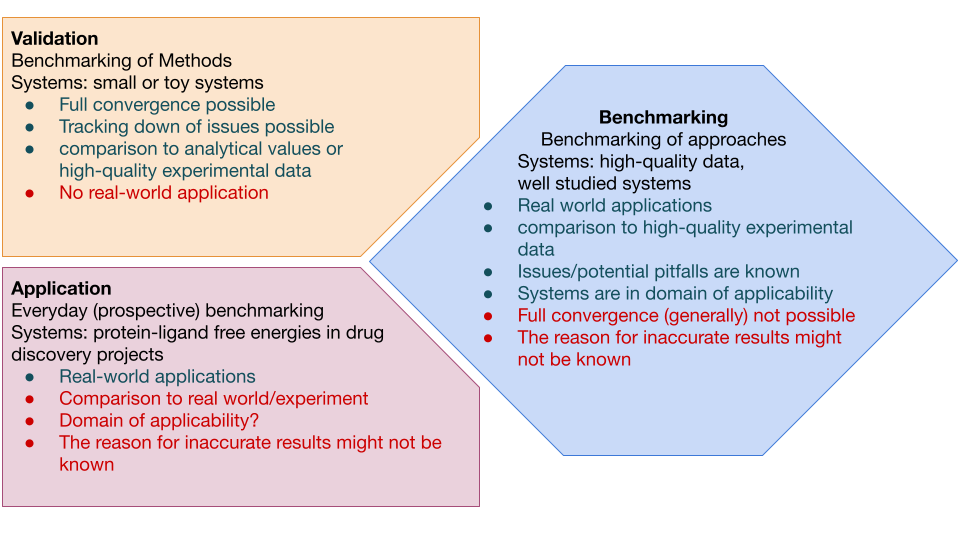
\includegraphics[width=0.95\linewidth]{figures/introduction/benchmarking_definition.png}
    \caption{\textbf{Illustration of the benchmark definition used in here}.}
    \label{fig:benchmarking_definition}
\end{figure*}

Drug discovery lead optimization (LO) typically involves the synthesis of hundreds of close analogues, often differing by only small structural modifications, in order to identify the optimal leads that show a good balance of target potency and other properties. This makes it an ideal scenario for RBFE where small differences in structure are well suited to alchemical perturbation. A number of recent studies have highlighted the good performance of RBFE for LO datasets. The high profile report from Wang et al.~\cite{wangAccurateReliablePrediction2015} used their commercial implementation of FEP and reported mean unsigned errors of < 1.2 kcal/mol. As they pointed out at the time, it is challenging to set up and reliably run RBFE calculations, but their results were robust over a relatively large dataset of 8 protein targets, 199 ligands, and 330 perturbations. It is not reported why these protein-ligand sets were chosen, other than they may be typical of current LO drug discovery. The same group has re-used this dataset to test updates to their force field (OPLS3\cite{harder_opls3_2016} and OPLS3e\cite{roos_opls3e_2019}). Today, this has become the de facto dataset for most large scale RBFE reports. It has been used to compare the performance of Amber/TI calculations~\cite{songUsingAMBER18Relative2019}, Flare’s FEP (Cresset and Michel group)~\cite{kuhnAssessmentBindingAffinity2020} and used as a subset with PMX and Gromacs\cite{gapsysLargeScaleRelative2020}. This dataset has also been used in machine learning studies~\cite{jimenezDEEPProteinLigand2018,jimenez-lunaDeltaDeltaNeuralNetworks2019}. In contrast, to date ABFE calculations have not been studied with datasets of a similar scale, although individual reports have shown success accurately predicting binding affinities~\cite{aldeghiLargescaleAnalysisWater2018,courniaRigorousFreeEnergy2020}.

Despite the success cases, there are many reports showing that RBFE calculations still struggle in certain scenarios,\cite{sherborne_collaborating_2016} such as with scaffold modifications~\cite{wangAccurateModelingScaffold2017} and ring expansion~\cite{liuRingBreakingFeasible2015}, water displacement\cite{michel_energetics_2009,brucemacdonald_ligand_2018,ross_enhancing_2020a,ben-shalom_accounting_2020}, protein flexibility\cite{huang_insights_2012,fratev_improved_2019,singh_absolute_2020}, applications on GPCRs\cite{lenselink_predicting_2016,deflorian_accurate_2020} and the modelling of cofactors like metal ions or heme (CITE). This is manifest in a large-scale study of FEP applied to drug discovery projects at Merck KGaA, in which Schindler et al. reported several cases of disappointing outcomes~\cite{schindler_largescale_2020}. In addition, new methods and implementation improvements for FE calculations continue to emerge, for instance the efforts on lambda dynamics~\cite{knightMultisiteDynamicsSimulated2011,vilseckPredictingBindingFree2018}, and non-equilibrium RBFE calculations~\cite{gapsysLargeScaleRelative2020,rufaChemicalAccuracyAlchemical2020}. Furthermore, there are many other methodologies such as end-point binding FE calculations (for instance MMGBSA, MMPBSA) or pathway based FE calculations that continue to be developed and applied. Therefore, we must balance the increased confidence that simulation-based FE calculations can impact drug discovery, with the need to further understand, test and overcome limitations of the current methods.

In brief, the issues mentioned above are related to three challenges or FE calculations,
(1) an accurate representation of the biological system, 
(2) an accurate force field, and 
(3) sufficient sampling. 
Therefore, despite the importance of FE methods to drug discovery and chemical biology it is surprising that there are no benchmark sets or standard benchmark methodologies that allow calculation approaches to be compared in a manner that will reflect their future performance. 

The Drug Design Data Resource\cite{_d3r_} (D3R) and Statistical Assessment of the Modeling of Proteins and Ligands\cite{mobley_sampl_} (SAMPL) prospective challenges have demonstrated the utility of focusing the community on common benchmark systems and using common methods to analyze performance\cite{geballe_sampl2_2010,muddana_blind_2012,muddana_prediction_2012,muddana_sampl4_2014,gathiaka_d3r_2016,bannan_blind_2016,yin_overview_2017,gaieb_d3r_2018,gaieb_d3r_2019,parks_d3r_2020}. Mobley and Gilson discussed the need for well-chosen validation datasets and how this will have multiple benefits to understand and expand the domain of applicability of FE methods~\cite{mobleyPredictingBindingFree2017}. They focused on validation systems that will confidently converge, and where the underlying issues are well understood, the aim was to describe systems that could be used only to assess method performance in a robust manner. As mentioned above, here we define benchmarking as assessing accuracy relative to experiment. This has implications that will be discussed in more detail throughout this article, for instance, the reliability of the underlying experimental data (structure and bioactivities), the confidence in the system setup such as protein and ligand preparation, are the alchemical perturbations suitable for FE, will the dataset be statistically powered, do datasets capture challenging real-world applications, and recommendations for analysing results. Essentially, we seek to understand what performance can be achieved when all these variables are handled to the best of our abilities.    

Here, our proposed benchmark set augments existing datasets while recommending cleaning up or removing entirely some protein-ligand sets. Here, we highlight key considerations in the construction of a useful set of protein-ligand benchmarks and the preparation of these systems for use as a community-wide benchmark. These recommendations are mirrored in a living benchmark set, which can be used to reliably launch future studies and which is provided on github.\cite{_openforcefield_2020}
%
We also recommend statistical analyses for assessing and comparing the accuracy of different methods and provide a set of open source tools that implement our recommendations.\cite{github_openforcefield_arsenic_2020} 
%
We hope these materials will become a common standard utilized by the community for assessing performance and comparing methodologies.  


\section{Prerequisites}
We assume a basic familiarity with molecular dynamics (MD) simulations, as well as alchemical free energy protocols. If you are unfamiliar with both of these concepts we suggest the best practices guides by Braun et al.~\cite{braunBestPracticesFoundations2019} on molecular simulations and Mey et al.~\cite{meyBestPracticesAlchemical2020} on alchemical free energy calculations as a starting point. 


%%%%%%%%%%%%%%%%%%%%%%%%%%%%%%%%%%%%%%%%%%%%%%%%%%%%%%%%%%%%
\section{Dataset Selection}
\label{sec:dataset}
%%%%%%%%%%%%%%%%%%%%%%%%%%%%%%%%%%%%%%%%%%%%%%%%%%%%%%%%%%%%

Details of our criteria for good benchmark datasets will follow throughout the rest of the manuscript. Here, we examine the purpose of protein-ligand benchmark datasets, and of expanding these sets.
We propose a core of robust datasets that match optimal criteria for benchmarking but suggest supplementing this core with new datasets which explore increasingly difficult concepts. A variety of parameters can guide future datasets.

%%%%%%%%%%%%%%%%%%%%%%%%%%%%%%%%%%%%%%%%%%%%%%%%%%%%%%%%%%%%
\subsection{Protein Selection}
\label{sec:dataset:proteins}
The selection and composition of target proteins in the benchmark set is generally dependent
on availability of experimental data and whether specific targets are in the domain of applicability.
%
It should be representative of classical drug discovery targets and chemistry, but still be diverse in terms of chemistry and targets. New additions should also reflect the evolution of drug discovery and the emergence of new target families.
% nuclear receptors, G protein-coupled receptors, ion channels, proteases, kinases, epigenetic targets, protein protein interactions, etc. 
Binding FE calculations are agnostic to protein classification, but there can be a pragmatic value in
expanding benchmark sets to new protein families that may present unexpected inherent difficulties (see Section \ref{sec:dataset:challenges}).
%
Most importantly, a certain quality of structural experimental data is required (see Section \ref{sec:struct_data})
and the structure should be adequately prepared for MD simulation input (Section \ref{sec:prep}).

%%%%%%%%%%%%%%%%%%%%%%%%%%%%%%%%%%%%%%%%%%%%%%%%%%%%%%%%%%%%
\subsection{Ligand Selection}
\label{sec:dataset:ligands}
% Number of data points
FE calculations are relatively costly in terms of computational effort. A certain number of data points, either activity measurements or activity differences, will be needed to empower subsequent statistical analyses, see later sections \ref{sec:affinities} and \ref{sec:analysis}. 
%To answer this, consider beta secretase (BACE), a common drug discovery target that already occurs in FE benchmark datasets. Given the vast number of patents, medicinal chemistry articles, and X-ray structures it could be possible to construct hundreds of BACE FE datasets containing several dozen ligands in each. These might have value for very specific applications, but will likely offer limited scientific insight about cross-target performance. This same holds true for other targets; often the amount of data available far exceeds that needed for benchmarking.
A suitable set of ligand structures should contain no ambiguities and should fall within the domain of applicability
of the particular free energy method used. 
In the case of chiral centers, the binding data should be available for the specific stereoisomer.
The stereochemistry, tautomeric and protonation states should be reliably assigned. 
%
We recommend to annotate potentially challenging issues when compiling benchmark sets as some issues are not supported by all
software packages. 
These challenging issues are 
charge changes, 
change of the location of a charge,
ring breaking,
changes in ring size, 
linker modifications,
change in binding mode and 
covalently bound ligands. 
%
If the ligand sets are sufficiently large, they can then be split into separate subsets (subsets with e.g. different ring sizes or different charges).
%
Ligand sampling can be problematic in some cases. Aromatic rings with asymmetric substitution will usually sample dihedral rotations freely in solvent but can become trapped in protein pockets during short FE simulations.\cite{kaus_how_2015} Macrocycles present more extreme issues of ligand sampling and likely require special consideration.\cite{wagner_computational_2017,yu_accurate_2017,paulsen_evaluation_2020} 
%The restrictions on charge states are preferable for comparative benchmarking of multiple FE methods, since methods for dealing with charge changes are not yet supported in all software packages. Similarly, transformations involving ring breaking and changes in ring size should be avoided at the moment (if a large enough number of molecules is available, these can be split into separate sets), as well as datasets with covalently bound inhibitors. 
% Note that e.g., the FEP+ method \cite{wangAccurateReliablePrediction2015} can support these types of transformations\cite{wangAccurateModelingScaffold2017,} and previously published benchmark sets \cite{{schindler_largescale_2020} also include such cases. 
The chemical diversity of the ligands that can be considered in a benchmark needs to be suitable for the given free energy method. Single RBFEs rely on common structural elements between the molecules being compared, and are hence more appropriate for a congeneric series of ligands. 
%
ABFEs are more amenable for comparing sets of small molecules where a change has been made to the scaffold. Similarity between ligands compared is also preferable if assumptions are being made about the binding mode of the ligand - which is tied to the quality, and availability of crystal structures of the system. If the data permitted, an ideal benchmark would be suitable to both absolute and relative free energy methods to allow comparisons.

% \begin{figure}
%     \centering
%     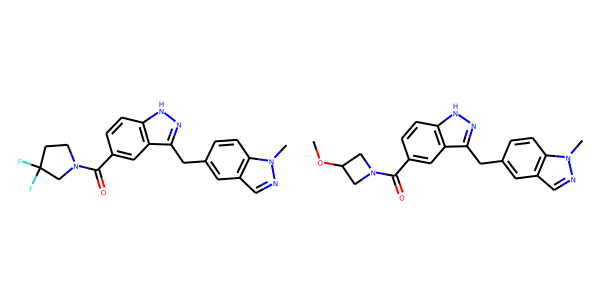
\includegraphics{cdk8.svg}
%     \caption{Caption}
%     \label{fig:my_label}
% \end{figure}
%%%%%%%%%%%%%%%%%%%%%%%%%%%%%%%%%%%%%%%%%%%%%%%%%%%%%%%%%%%%
\subsection{Addressing specific challenges}
\label{sec:dataset:challenges}

Besides the challenges mentioned in Sections \ref{sec:dataset:proteins} and \ref{sec:dataset:ligands},
there are specific challenges which can be addressed by a benchmark set. These include 
water displacement in binding sites,
the presence of cofactors in the binding site, 
slow motions of ligands (e.g. rotatable bonds) and proteins, and 
activity cliffs.
We recommend to annotate these challenging cases in the benchmark set.

%%%%%%%%%%%%%%%%%%%%%%%%%%%%%%%%%%%%%%%%%%%%%%%%%%%%%%%%%%%%






% Choosing an appropriate test system is the first step in validating free energy methods. Factors to consider fall into two overarching categories: quality of the structural data, and quality of the affinity data. The perfect experimental data would be such that if any discrepancy between experiment and computational prediction could be blamed on the computational prediction, and therefore could be blamed on any of the flogging posts of computational chemistry: insufficient sampling, buggy algorithms or poor forcefields.
% Common data sources (structural and binding data, prepared for simulations):
% Requirements (https://agilescientific.com/blog/2019/4/3/what-makes-a-good-benchmark-dataset)
% Publicly available
% Sustainable, long-term
% Easy to use/retrieve
% Interesting (‘Approved by the community’)
% Consistent and high quality data
% Clean
% Documented

% List of common data sources (what do they contain, is the information complete?):
% BindingDB
% Drug Design Data (D3R) Challenges: https://drugdesigndata.org/
% Wang et. al, Schrodinger
% Gapsys et al., Large scale relative protein ligand binding affinities using non-equilibrium alchemy
% Schindler et al., Merck KgGA, fep-benchmark, and associated publication
% Perez-Benito et al., Janssen, Prediciting Activity Cliffs with FEP
% SiliconTx Benchmarks

%-----------------------------------------------------------
\subsection{Structural Data}
\label{sec:struct_data}
%-----------------------------------------------------------

% Source of structure (crystallography/CryoEM/NMR).
% Content of the structure: is the small molecule (or a closely related one) bound? Are there cofactors or cobinders?
% Conditions of structure measurement: temperature, ion concentration, other additives?
% Resolution of the structure:
% Global metrics such as R2 can give an indication of the structure
% Are there crystal contacts? Can you assume the structure in the crystalline form is representative of the biologically active conformation
% Are there missing side chains or residues, or multiple configurations present? Are the termini biologically correct?
% Local resolution: is the active site clearly defined? Is the electron density for the ligand (if there is one) clear? Also are crystallographic waters resolved? Local metrics such as EDIA or Zobs or Spruce(?) can indicate if the electron density is sufficient to support the crystallographic placement of a given atom.
% Iridium publication from Greg Warren, source of a checklist of things to care about: https://doi.org/10.1016/j.drudis.2012.06.011
% Zoe Woody Bryce -- Relative paper in JCIM, things to keep in mind when you’re preparing a protein.

A successful free energy calculation requires a well prepared accurate model of the system to be simulated, with structure(s) representative of the equilibrium state of the system. Just as choices made selecting binding data are critical, the choices made when selecting a protein model will have an impact on benchmarking.
%
Often structural studies use shorter constructs that might be missing several domains compared to the full-length protein. To facilitate crystallization or expression, mutations might have been introduced. In addition, parts of the protein might not be resolved or modelled. Ideally, such deviations should be kept to a minimum in a benchmark data set.
%

Starting structures are typically obtained from experimentally constrained models, most commonly obtained from X-ray diffraction data.
Other sources include cryo-EM, NMR or homology models.
%https://doi.org/10.1021/acs.jcim.7b00564, %https://doi.org/10.1021/acs.jcim.0c00116; %https://doi.org/10.26434/chemrxiv.11364884.v2; 
As free energy calculations are usually run at atomic resolution, the input structure needs to provide the coordinates of all atoms ideally determined by the experimental model.
%
For X-ray and cryo EM structures, this requirement is only met by high quality structures.
The evaluation criteria defined by OpenEye Iridium\cite{warrenEssentialConsiderationsUsing2012} can guide the assessment of X-ray structure. It is important to note that the Iridium criteria were designed to assess structures for benchmarking docking and not necessarily for free energy. As such there is one important criteria missing - completeness of the model.


Any protein structural assessment should be done using two filters; overall (global) and local. Traditionally, overall quality of the structure (global) had been assessed using X-ray or cryo EM resolution as it is easily accessible.
%
However, this metric is a theoretical limit and does not assess the quality of the model. Therefore, it is not a good metric for accuracy, completeness or quality and should only be used alongside other metrics. Iridium, by design, does not set a resolution limit but suggests a resolution threshold of $< 3.5\,\AA$,\cite{warrenEssentialConsiderationsUsing2012} because it is difficult to model side chain atoms precisely above that criteria. Stricter thresholds have been suggested (i.e. $<2.0\,\AA$  in a recent benchmark\cite{schindler_largescale_2020}).
%
More meaningful metrics for X-ray are $R$, $R_{\mathrm{free}}$ and the coordinate error. Currently, equivalent metrics for cryo-EM structures either do not exist or are less well understood.  As a result the rest of the discussion will focus on criteria for structures determined using X-ray or neutron diffraction data.  It should be noted that cryo-EM maps can still be visualized with the model to get a idea of the agreement between the model and the data.
%
The $R$-factor is a measure for the difference between the predicted data (by the model) and the measured data. A smaller $R$-factor indicates an experimentally consistent model. A complication with $R$-factor is that it is a non-normalized metric. For a given data set the model with the lowest $R$-factor is best fit to the data.  Unfortunately, for different data sets, even for the same protein, lowest $R$-factor may not be the highest quality model. 
%
The $R_{\mathrm{free}}$-factor is calculated the same way, but uses only a held out randomly selected subset of the measured data. Thus, it can be used to identify overfit models which will be apparent in a larger difference between $R$-factor and $R_{\mathrm{free}}$ (typically more than 0.05).
Both $R$-factors are easily accessible for reported crystallographic data, e.g. in the protein data bank (PDB).\cite{bermanProteinDataBank2000} 
%
While more difficult to find or calculate, the best way to assess the precission and quality of the model, is the coordinate error metric,
%
\begin{equation}
    \mathrm{coordinate\ error} = \frac{2.22 R_{\mathrm{free}}\sqrt{N_i^3}\sqrt{V_a}} {n_{\mathrm{obs}}^{5/6}},
    \label{eq:coordinate_error}
\end{equation}
%
where $N_i$ is the number of heavy atoms with occupancy of 1, $V_a$ is the volume of the asymmetric unit cell and $n_{\mathrm{obs}}$ is the number of non-$R_{\mathrm{free}}$ reflections used during refinement. A high-quality structure should have a coordinate error $<0.7$. Resent PDB entries usually include a coordinate error estimate which can be found by searching for ESU $R_{\mathrm{free}}$, Cruickshank or Blow Density Precision Index (DPI). Coordinate error (as shown in Equation 1) is $\sqrt{3}\mathrm{BlowDPI}$. 

\begin{landscape}
\begin{table*}[ht]
\caption{
Evaluation of the quality of structural and activity experimental data of the proposed benchmark set.
%
The successive entries are the 
target name/identifier,
the used PDB ID and its quality evalutation in terms of
Iridium classification (Ir. Class.), 
Iridium score (Ir. Score) and 
diffraction-component precision index (DPI).
%
The structures listed in "Used structure" are those used in the initial version of this dataset, which is drawn in part from previous studies. However, alternate available structures may be superior. In these cases, we provide a PDB ID of a higher quality structure and 
its quality measures, in the "Alternate structure" fields.
%
Regarding activity data ("Ligand Information"), the number of ligands (count), the dynamic range ($\mathrm{max}(\Delta G)-\mathrm{min}(\Delta G)$) and the standard deviation of the $\Delta G$ ($\mathrm{std}(\Delta G)$) is given.
}
\label{tab:struct}
\begin{tabular}{l|llll|lll}
Target     & \multicolumn{4}{c|}{Used structure}                          & \multicolumn{3}{c}{Alternate structure} \\
           & PDB ID      & Ir. Class. & Ir. Score & DPI  & PDB ID & Ir. Class. &  Ir. Score\\
\hline
BACE(Sch)   & 4DJW        & HT                     & 0.32          & 0.11 & 6UWP& HT& 0.28\\
BACE(HUNT1) & 3ZOV        & MT                     & 0.4           & 0.2  & 6UWP& HT& 0.28\\
BACE(HUNT2) & 4JPC        & HT                     & 0.32          & 0.12 & 6UWP& HT& 0.28\\
BACE(P2)    & 3IN4        & HT                     & 0.59          & 0.28 & 6UWP& HT& 0.28\\
CDK2       & 1H1Q        & MT                     & 0.87          & 0.28 & 3DDQ& HT& 0.31\\
CDK8       & 5HNB        & MT                     & 0.74          & 0.22 & 5XS2& HT& 0.33\\
EG5        & 3L9H        & MT                     & 0.88          & 0.18 & 2X7C& HT& 0.32\\
Galectin   & 5E89        & MT                     & 1.04          & 0.07 & 5NF7& HT& 0.3 \\ 
HIF2a      & 5TBM        & HT                     & 0.35          & 0.17 & 3H82& HT& 0.3 \\ 
Jnk1       & 2GMX        & NT                     & See Fig X     & 0.77 & 3ELJ& MT& 0.31\\
MCL1       & 4HW3        & HT                     & 0.41          & 0.26 & 6O6F& HT& 0.3 \\
P38(MAPK14)& 3FLY        & HT                     & 0.6           & 0.12 & 6SFI& HT& 0.3 \\
PDE2       & 6EZF        & MT                     & 0.3           & 0.07 & 6C7E& HT& 0.29\\
PFKFB3     & 6HVI        & HT                     & 0.31          & 0.11 & & & \\
PTP1B      & 2QBS        & MT                     & 0.33          & 0.15 & 2HB1& HT& 0.32\\
SHP2       & 5EHR        & MT                     & 0.32          & 0.1  & 6MD7& HT& 0.35\\
SYK        & 4PV0        & MT                     & 0.69          & 0.19 & 4PX6& HT& 0.3\\
Thrombin   & 2ZFF        & HT                     & 0.3           & 0.06 & 5JZY& HT& 0.27\\
TNKS2      & 4UI5        & HT                     & 0.29          & 0.08 & 4BU9& HT& 0.29\\
TYK2       & 4GIH        & HT                     & 0.5           & 0.15 & 3LXP& HT& 0.31\\
\end{tabular}
\end{table*}
\end{landscape}

\begin{figure}
    \centering
    \begin{subfigure}[b]{0.48\textwidth}
        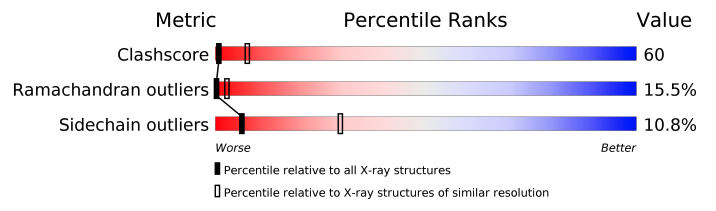
\includegraphics[width=\textwidth]{crystal/Jnk1_2gmx_pdb_report.png}
        \caption{}
        \label{fig:jnk1_pdb_report_2gmx}
    \end{subfigure}
    
    \begin{subfigure}[b]{0.48\textwidth}
        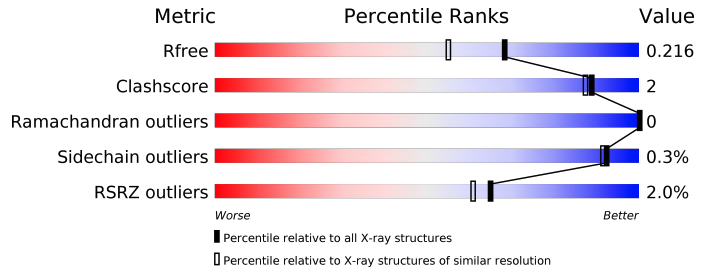
\includegraphics[width=\textwidth]{crystal/Jnk1_3elj_pdb_report.png}
        \caption{}
        \label{fig:jnk1_pdb_report_3elj}
    \end{subfigure}
    \caption{The PDB structure validation report percentile score figures for the Jnk1 structures 2GMX and 3ELJ.  Note that 2GMX (panel \subref{fig:jnk1_pdb_report_2gmx}) is a poorly ranked structure relative to all and structures of similar resolution in the PDB.  In contrast 3ELJ (panel \subref{fig:jnk1_pdb_report_3elj}) is at or better than structures of similar resolution or all structures in the PDB.}
    \label{fig:jnk1_pdb_report}
\end{figure}

While understanding the global quality of a structure is important it is the local active or ligand binding site that will have the largest impact on benchmarking performance. Thus special care should be taken to asses the ligand and surrounding the active site residues. 
%
Of highest priority is to identify all unmodeled residues and side chain atoms within 6 to $8\,\AA$  of any ligand atom. When multiple structures with similar coordinate error exist structure with no missing residues or side chain atoms that meet subsequent criteria should be used.
%
The electron density around the ligand should cover at least 90\% of the ligand atom centers, which can be checked visually or using a RSCC value $>0.90$ (see Figures 3c and 4d). Ligand atoms where there are crystal packing atoms within $6\,\AA$ should be identified (see Figure 3e). 
%
All ligand and active site atoms with occupancy <1.0 should be identified.
%
If there is only partial density for the ligand and the active site residue atoms, these partial-density atoms should be identified (see Figure 3c). If alternate conformations for the ligand or active site residues exist which conformation to use should be determined by looking at the electron density (see Figure 3a). Local metrics such as EDIA or a number of RSCC calculators can indicate if the electron density is sufficient to support the crystallographic placement of a given atom.
%
Covalently bound ligands should be identified and appropriately modelled.
%Local metrics such as EDIA or Zobs or Spruce(?) can indicate if the electron density is sufficient to support the crystallographic placement of a given atom.


\begin{figure*}
    \centering
    \begin{subfigure}[b]{0.48\textwidth}
        \centering
        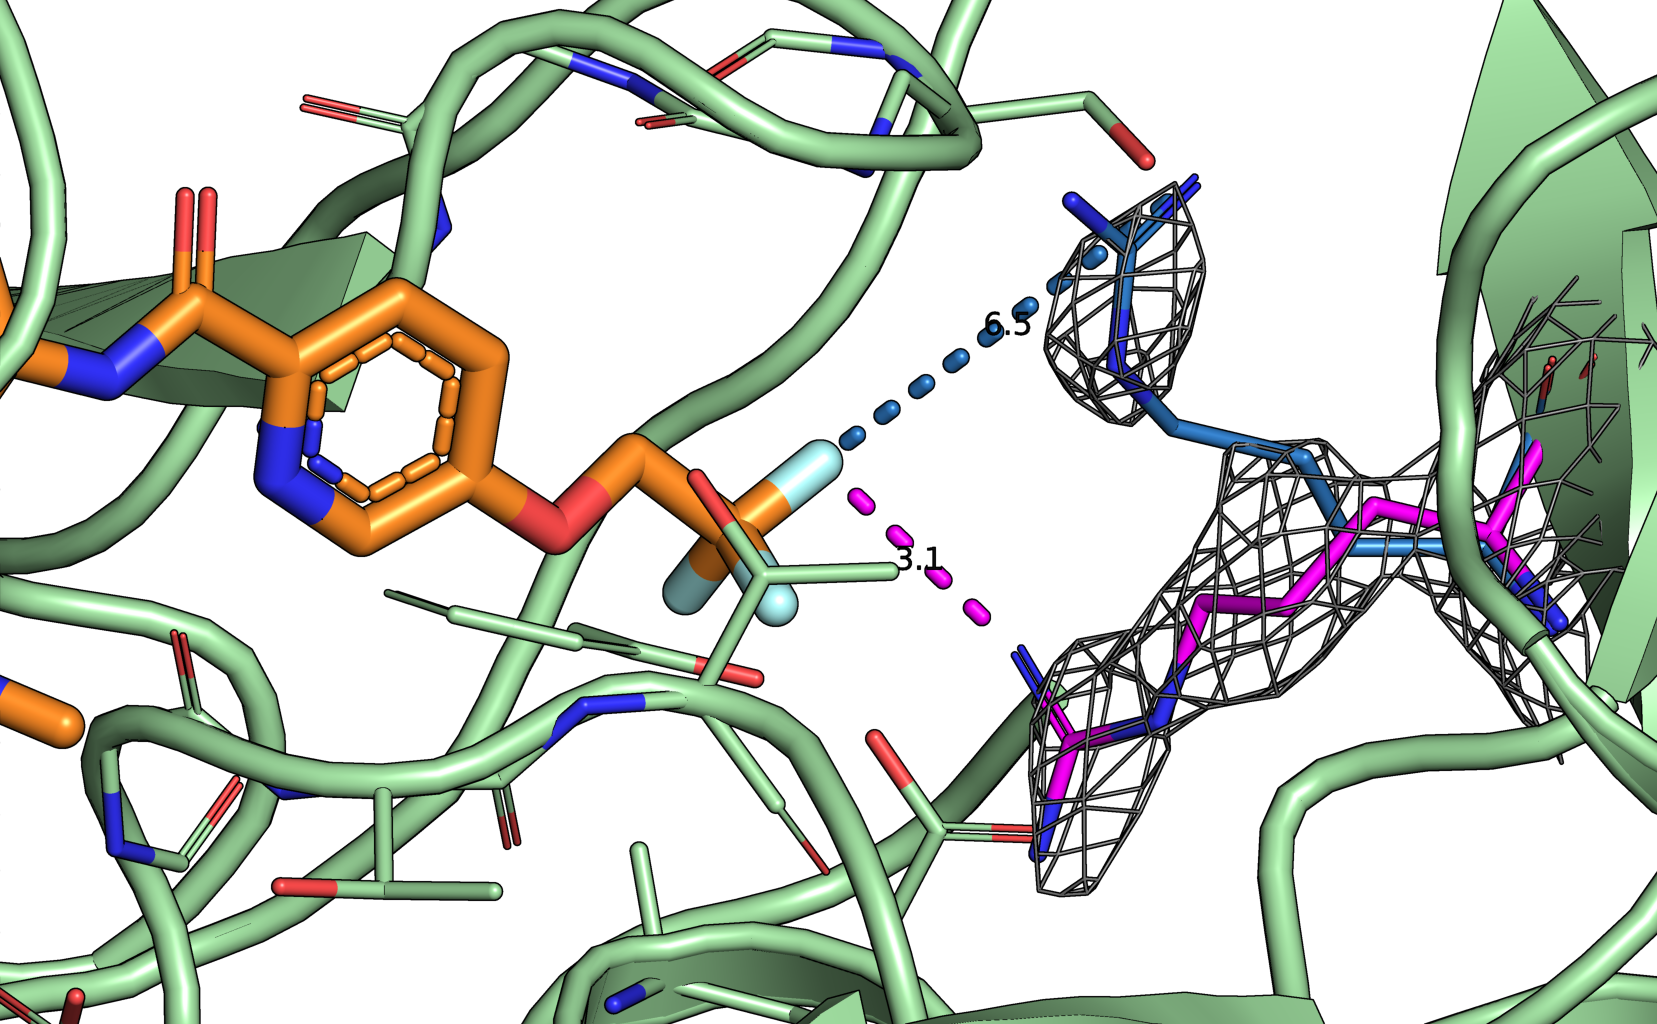
\includegraphics[width=\textwidth]{figures/crystal/pic_3zov.png}
        \caption{BACE (Hunt), PDB 3ZOV}
        \label{fig:3zov}
    \end{subfigure}
    \hfill
    \begin{subfigure}[b]{0.48\textwidth}
        \centering
        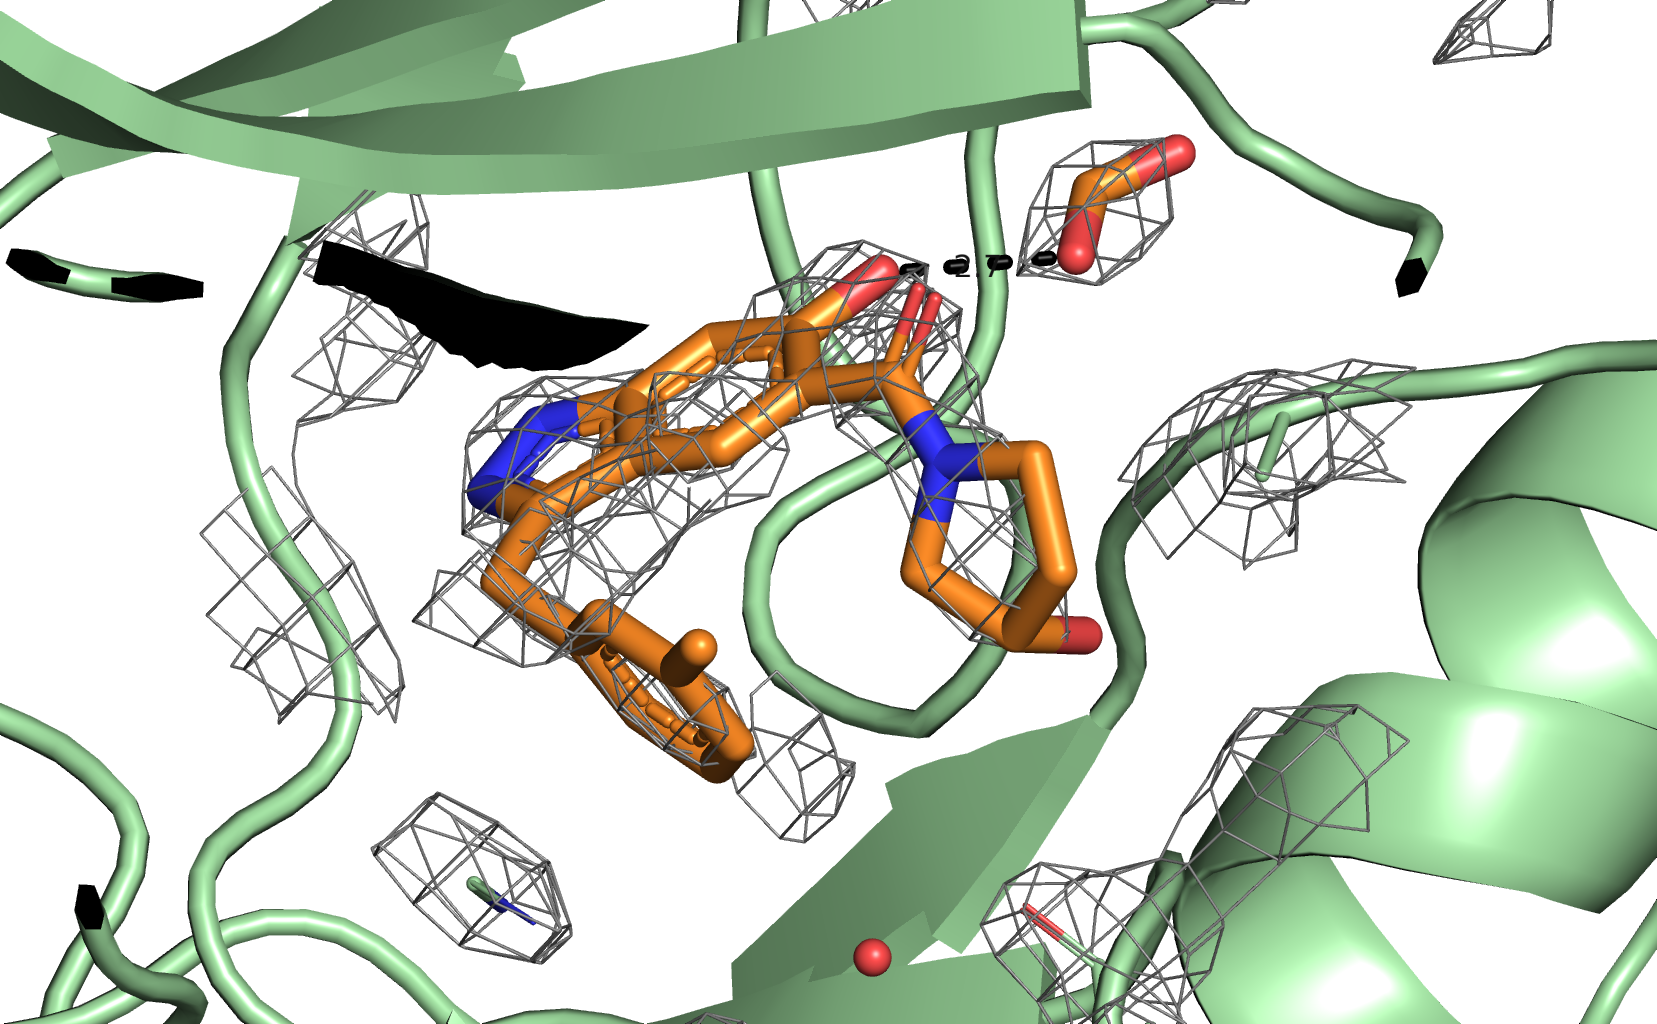
\includegraphics[width=\textwidth]{figures/crystal/pic_5hnb.png}
        \caption{CDK8, PDB ID 5HNB}
        \label{fig:5hnb}
    \end{subfigure}
    
    \begin{subfigure}[b]{0.48\textwidth}
        \centering
        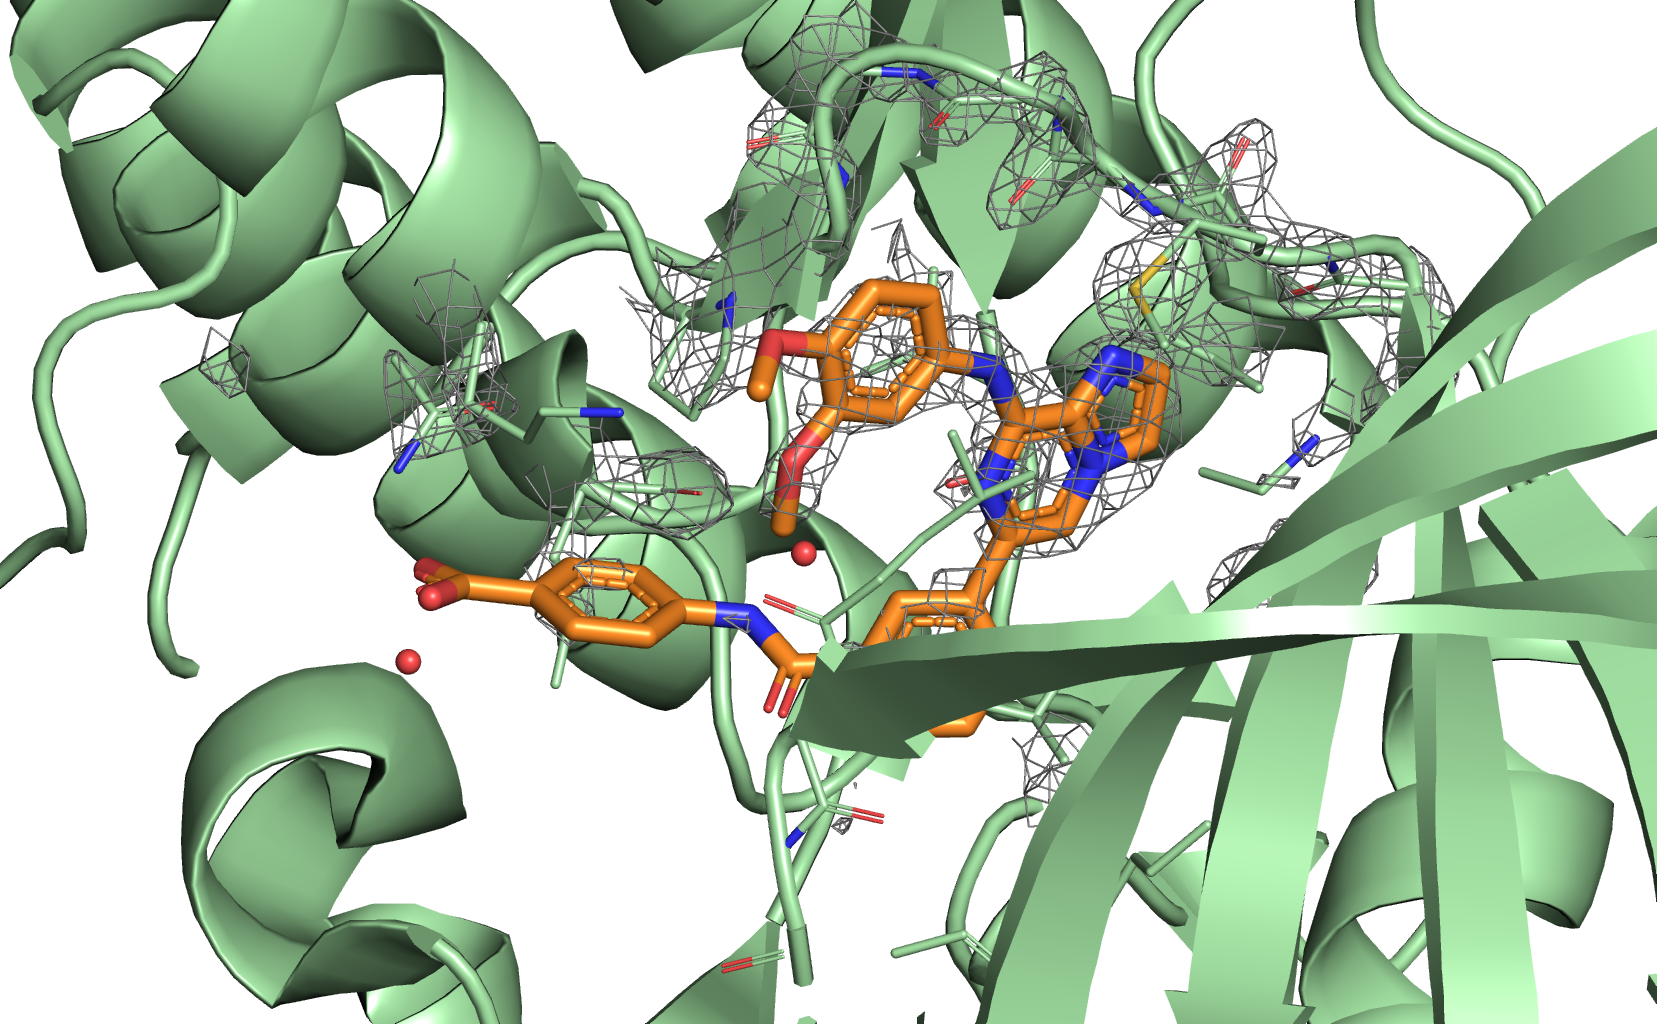
\includegraphics[width=\textwidth]{figures/crystal/pic_4pv0.png}
        \caption{SYK, PDB ID 4PV0}
        \label{fig:4pv0}
    \end{subfigure}
    \hfill
    \begin{subfigure}[b]{0.48\textwidth}
        \centering
        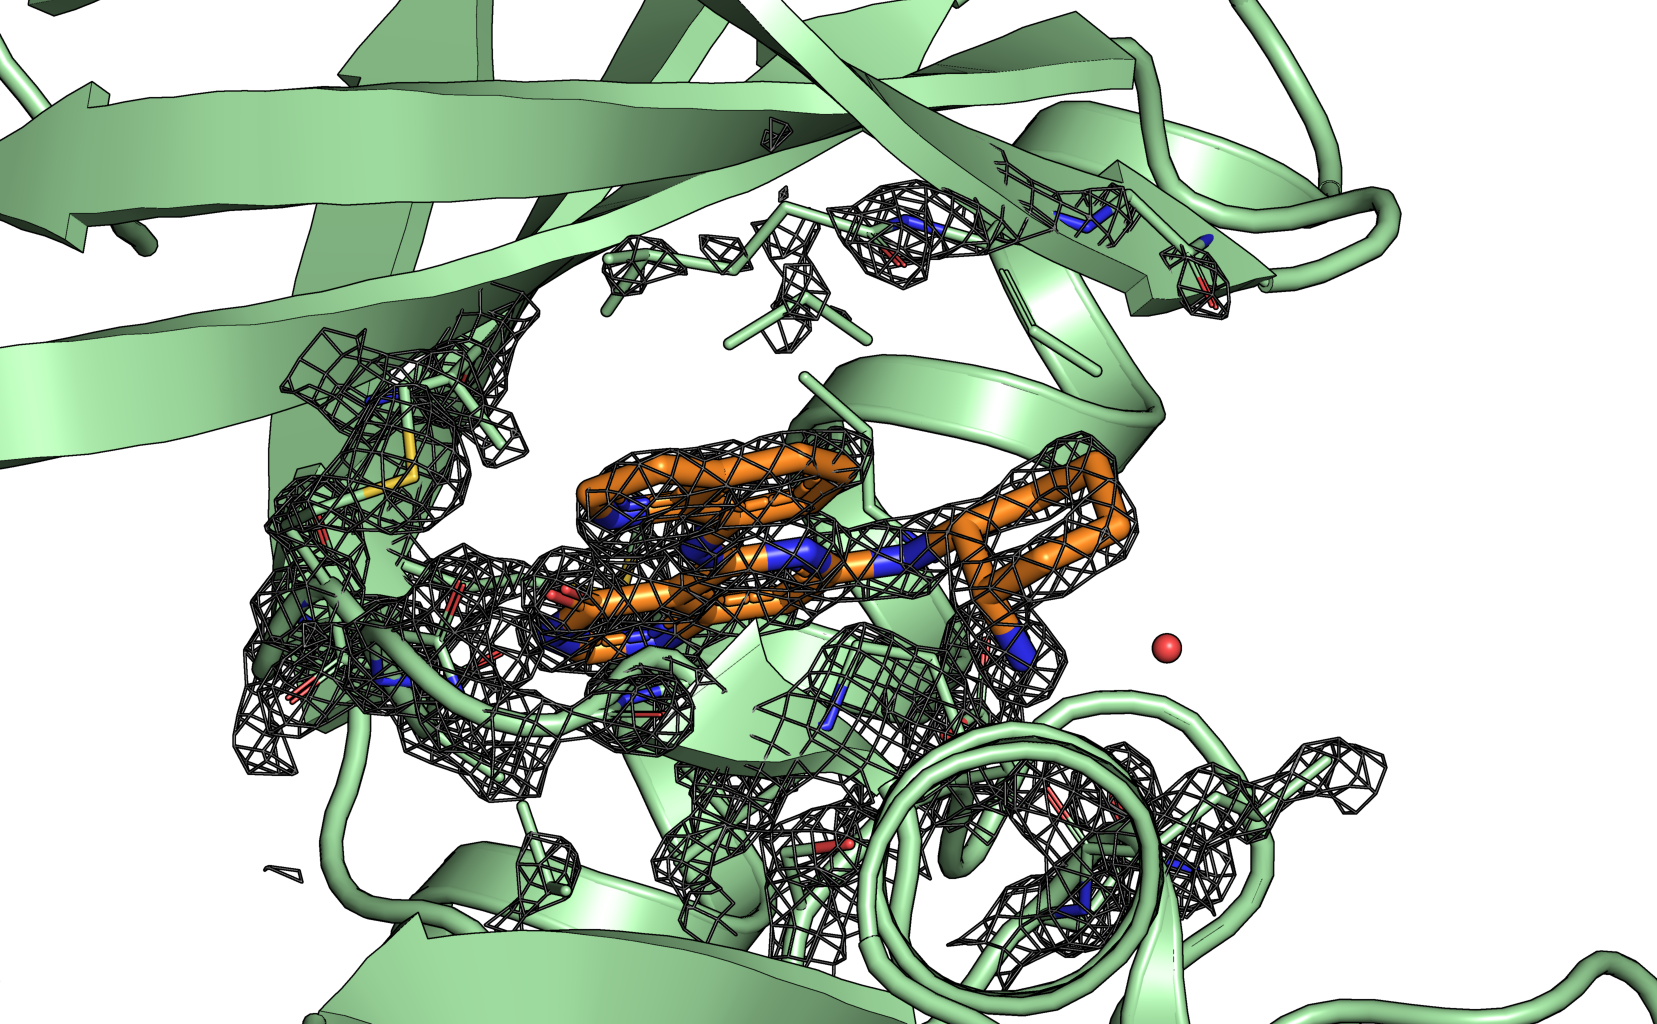
\includegraphics[width=\textwidth]{figures/crystal/pic_4px6.png}
        \caption{SYK, PDB ID 4PX6}
        \label{fig:4px6}
    \end{subfigure} 
    
    \begin{subfigure}[b]{0.48\textwidth}
        \centering
        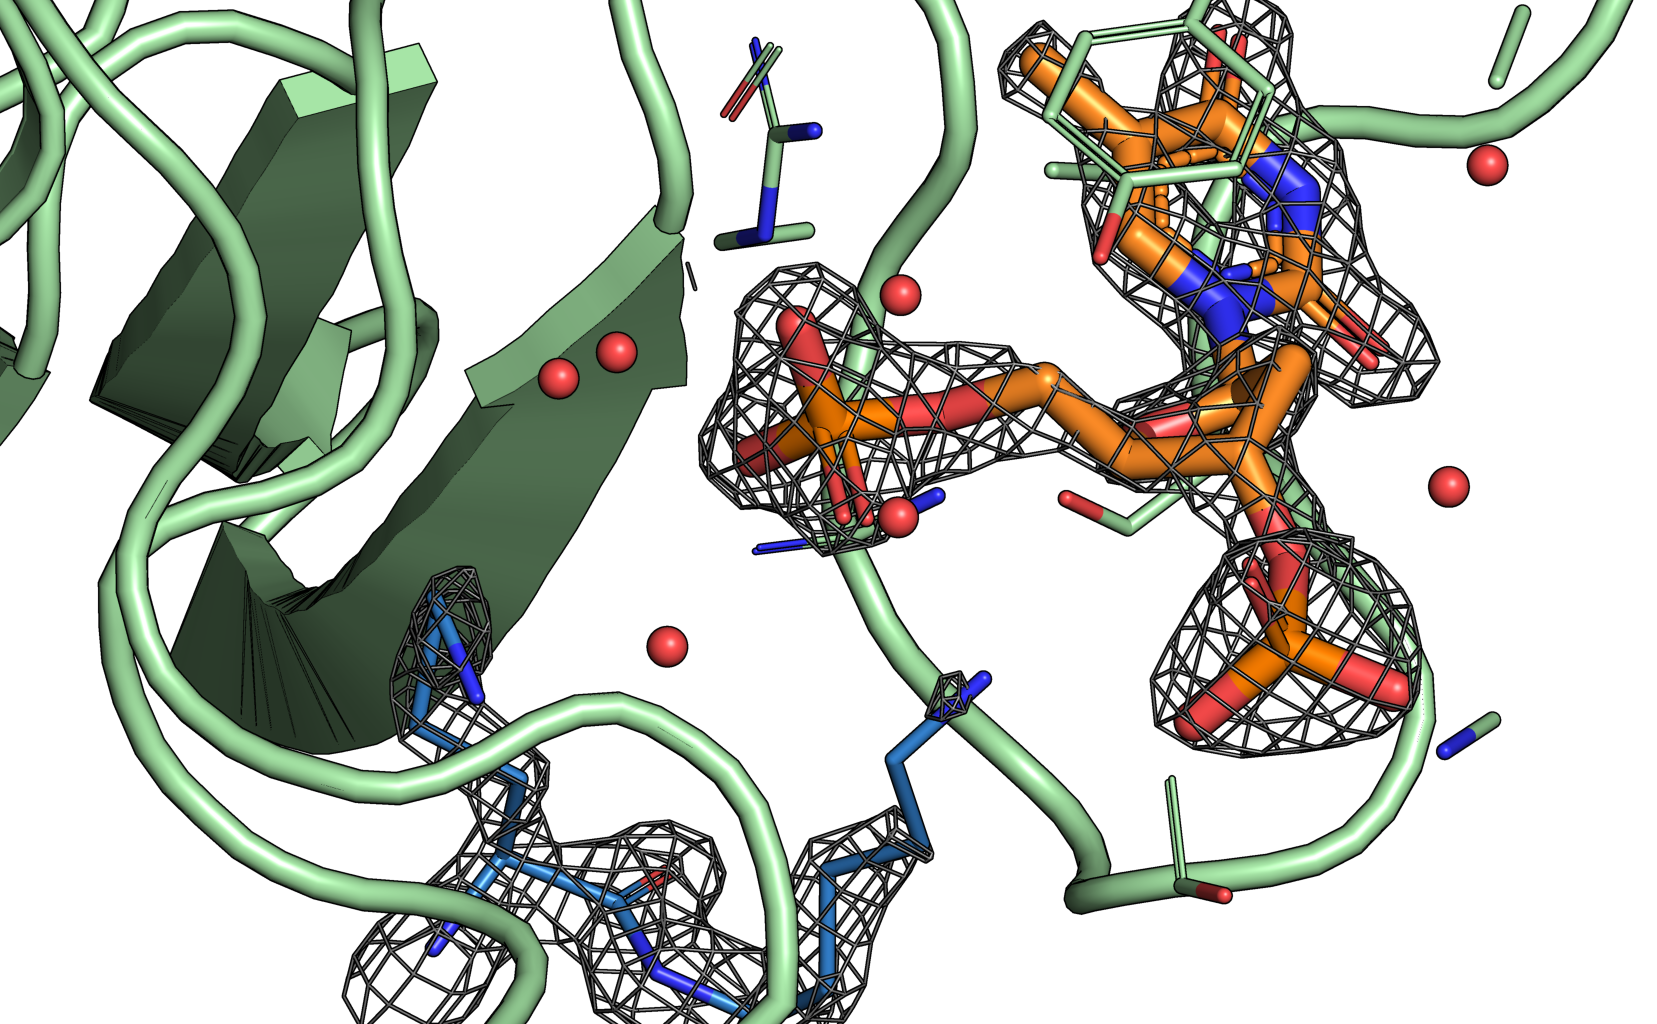
\includegraphics[width=\textwidth]{figures/crystal/pic_1snc.png}
        \caption{Staphylococcal nuclease, PDB ID 1SNC}
        \label{fig:1snc}
    \end{subfigure}
    \hfill ~\\
    
    \caption{Examples of challenges in X-ray crystal structures. The protein is shown in green and the ligand in orange. If not stated differently, the 2Fo-Fc maps are illustrated as grey isomesh at $2\sigma$ level. 
    %
    Panel (\subref{fig:3zov}): PDB ID 3ZOV has two
    alternate side chain conformations. Residue R368  in the B conformation (magenta) has clearly more density (0.75 $\sigma$) than the A conformation (blue). The B conformation interacts with the ligand (distance $3.2\,\AA$) whereas the A conformation does not interact with the ligand (distance $6.5\,\AA$). If the user does not look at both conformations and chooses A (by default) that would be an incorrect decision.  
    %
    Panel (\subref{fig:5hnb}): In PDB ID 5HNB, there is an excipient (formic acid) that interacts directly with the ligand ($2.7 \AA$ O-O distance shown in black).  The formic acid could be replacing a bridging water.  From the data it is not possible to determine how the excipient is affecting the ligand/protein conformation.
    %
    Panel (\subref{fig:4pv0}): PDB ID 4PV0  shows poor density for residues in the active site.  The beta sheet loop at the top of the active site has residue side chains modeled with no density to support the conformation and the end of the loop has residues that are not modeled.  
    %
    Panel (\subref{fig:4px6}): The recommended structure PDB ID 4PX6 for the same protein  has complete density (and modeled atoms) for the whole loop.
    %
    Panel (\subref{fig:1snc}): The ligand of PDB ID 1SNC has crystal contacts with the residues K70 and K71 (blue) of the neighboring unit that directly interact with the ligand.
    }
    \label{fig:crystal1}
\end{figure*}

\begin{figure*}
    \centering
    \begin{subfigure}[b]{0.48\textwidth}
        \centering
        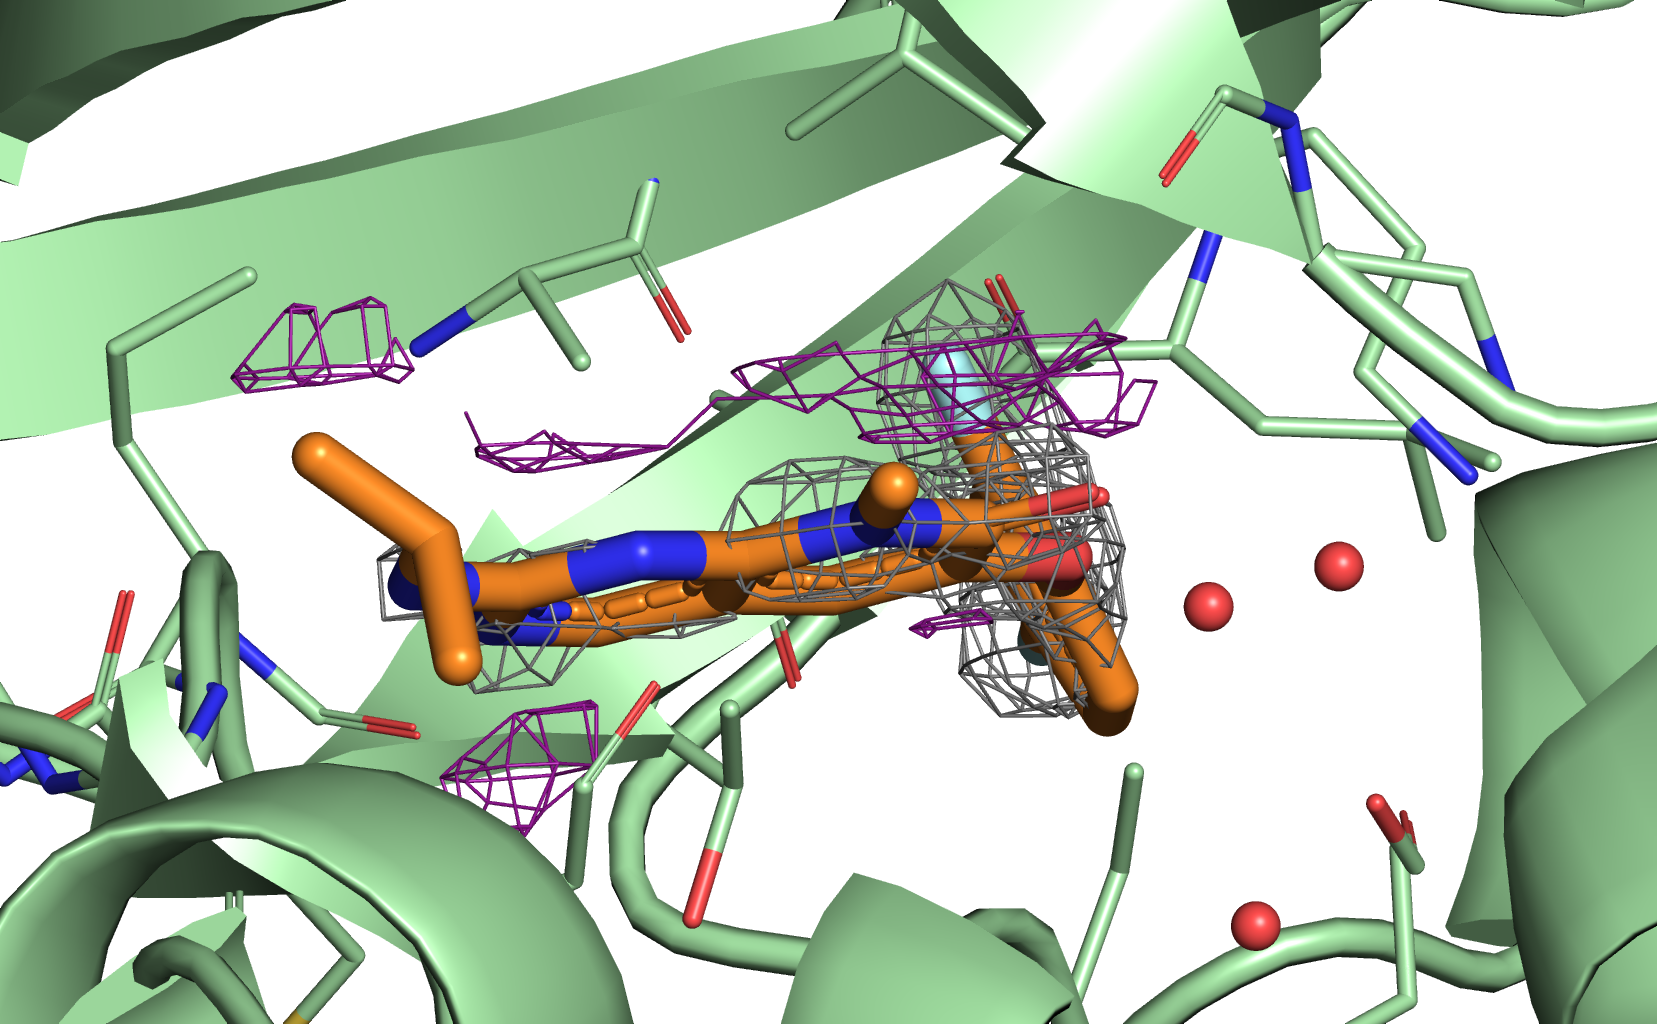
\includegraphics[width=\textwidth]{figures/crystal/pic_3fly.png}
        \caption{P38, PDB ID 3FLY}
        \label{fig:3fly}
    \end{subfigure}
    \hfill
    \begin{subfigure}[b]{0.48\textwidth}
        \centering
        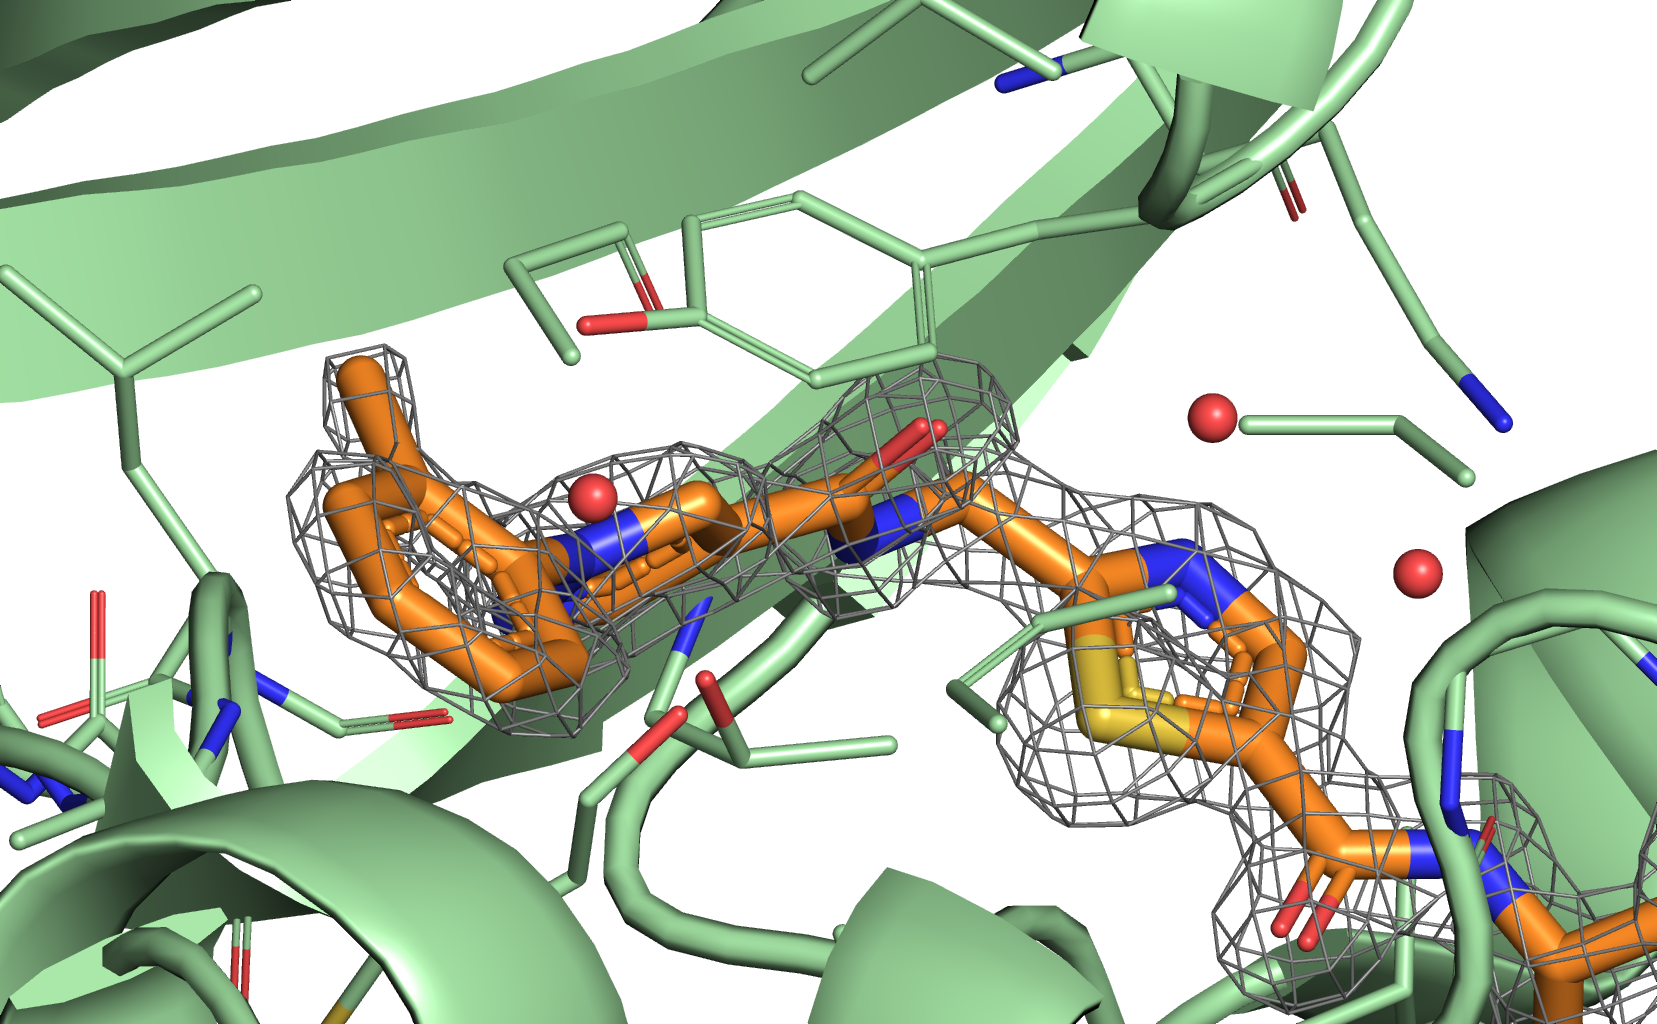
\includegraphics[width=\textwidth]{figures/crystal/pic_6sfi.png}
        \caption{P38, PDB ID 6SFI}
        \label{fig:6sfi}
    \end{subfigure}  
    
    \begin{subfigure}[b]{0.48\textwidth}
        \centering
        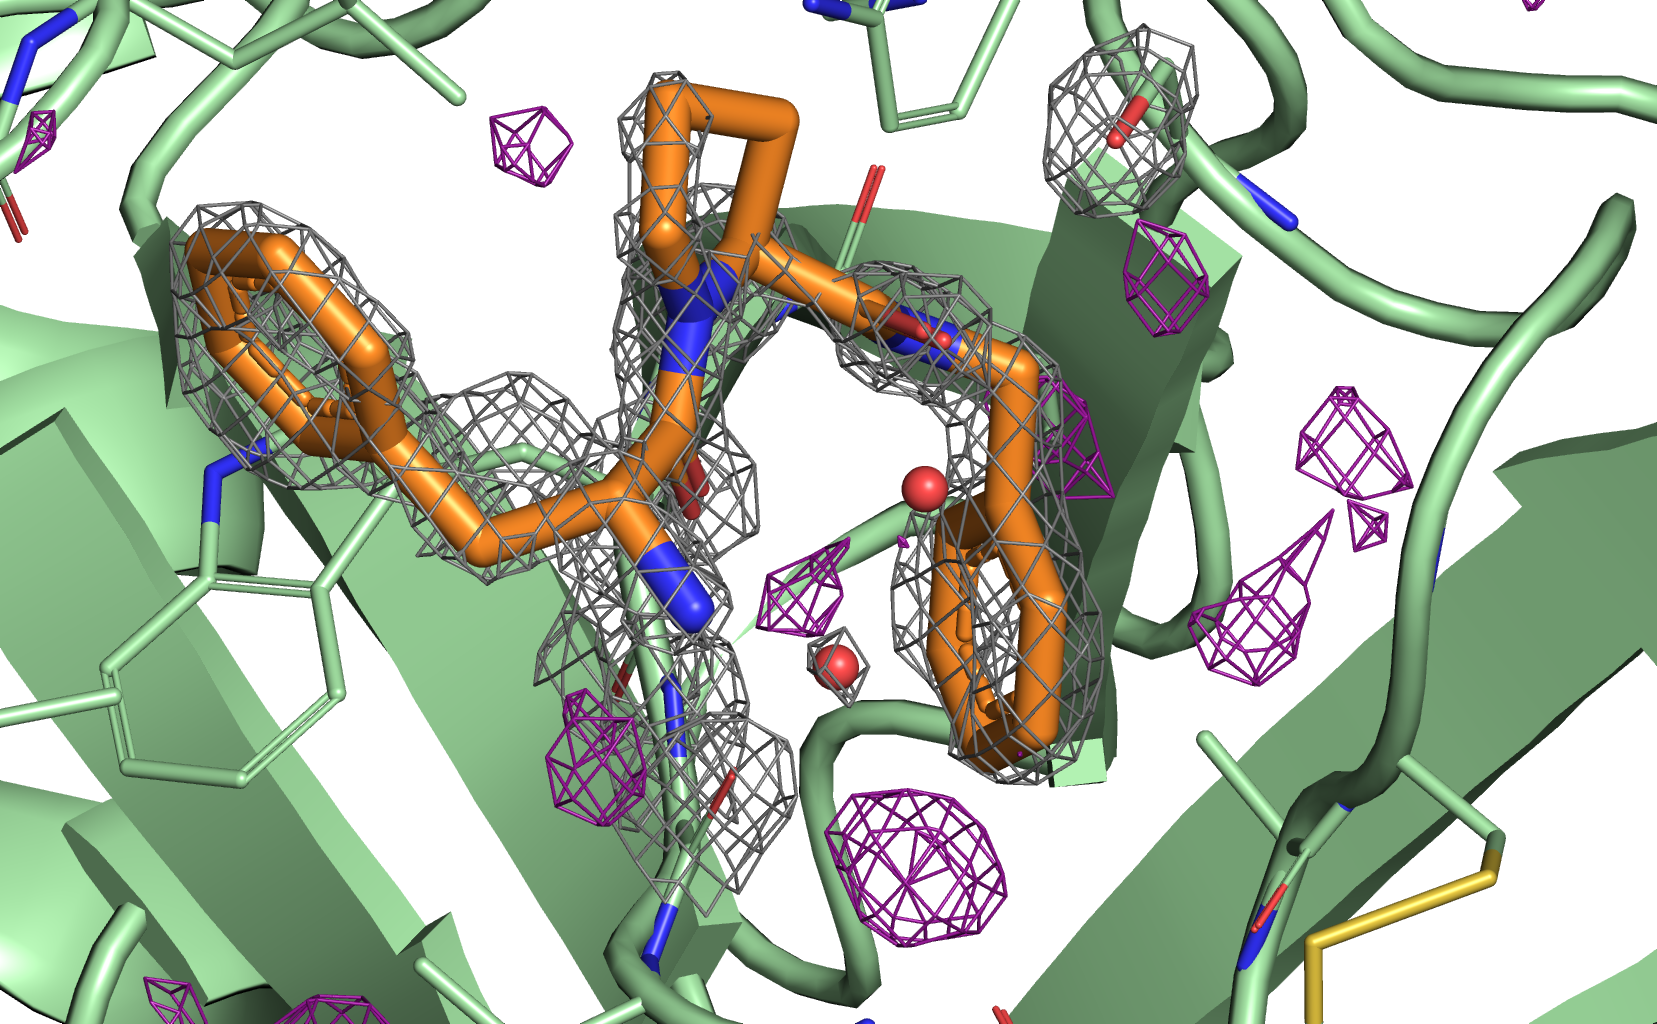
\includegraphics[width=\textwidth]{figures/crystal/pic_2zff.png}
        \caption{Thrombin, PDB ID 2ZFF}
        \label{fig:2zff}
    \end{subfigure}
    \hfill
    \begin{subfigure}[b]{0.48\textwidth}
        \centering
        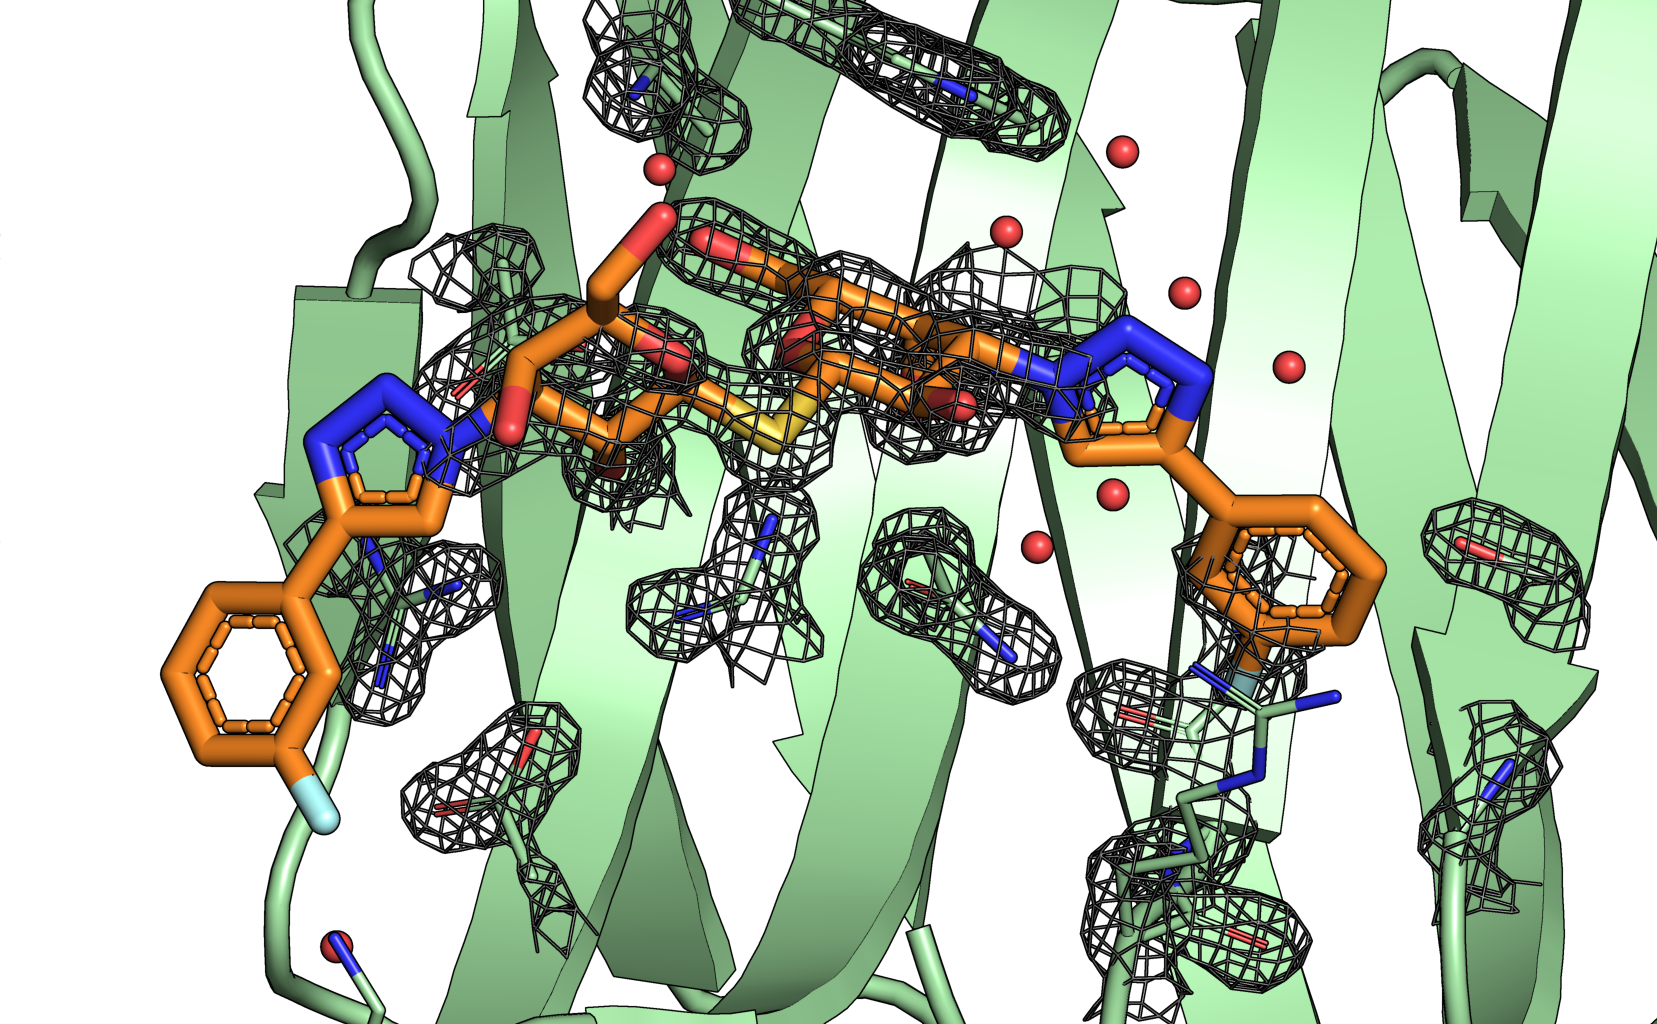
\includegraphics[width=\textwidth]{figures/crystal/pic_5e89.png}
        \caption{Galectin, PDB ID 5E89}
        \label{fig:5e89}
    \end{subfigure}      
    
    \caption{Issues regarding the ligand modelling in X-ray crystal structures. The protein is shown in green and the ligand in orange. If not stated differently, the 2Fo-Fc maps are illustrated as grey isomesh at $2\sigma$ level. 
    %
    Panel (\subref{fig:3fly}): In PDB ID 3FLY, there is difference density indicating that the ligand conformation is not modeled correctly.  It is suspected that there is a low occupancy alternate conformation that is not modeled.
    %
    Panel (\subref{fig:6sfi}): The suggested alternate structure of the same protein, PDB ID 6SFI, has no difference density.
    %
    Panel (\subref{fig:2zff}): PDB ID 2ZFF shows unexplained electron density in the binding pocket (difference map, bottom, center, purple). This could
    be either water or a $Na^+$ ion as $Na^+$ is present and modeled in other sites. 
    %
    Panel (\subref{fig:5e89}): PDB ID 5E89 shows poor ligand density, especially for the \textit{m}-Cl-phenyl (left) and the hydroxymethyl (center). This means that the ligand conformation, as shown, is not specified by the data.
    }
    \label{fig:crystal2}
\end{figure*}

Additional aspects should be considered beyond the quality of the model and the data (see also structure preparation, Sect. \ref{sec:prep}).
%
The structure of a complex could be deformed due to crystal contacts
or by experimental conditions like additives, pressure or temperature. These conditions might not be representative for the biological environment and therefore biologically active conformation of the complex. 
% what can we do about it?
%
Important for the active conformations could be crystal waters, co-factors or co-binders which should be included to model the natural environment of the protein (see Figure 3b and 4c). It is also important to remember that for X-ray data modeling water (versus amino acids or organic compounds) is less precise than for other atoms particularly when the crystal is formed in a high salt environment.
%
The ligand in the experimental structure should be sufficiently close to the ligand to be simulated to have a model of the correct binding mode. 
%
A choice of the simulation conditions like temperature, ion concentration, other additives like co-factors or membranes require additional considerations. Ideally, these conditions are close to structural experiment, the affinity measurements and the physiological conditions. Most likely, a trade-off between all of these has to be found. Where possible select structures where data was collected at room temperature that were crystallized using non-salt precipitants. Be aware that room temperature data will have lower precision and more conformational heterogeneity.
    
%
If these requirements are not met, it does not necessarily mean that the data is not usable and the results will be bad. A structure not meeting the requirements may suffice after more manual intervention by the user, ideally an experienced one. Unresolved areas can be modelled with current tools and knowledge about atom interactions, though this can be a cause for concern if these are near the binding site. This concern has been validated, at least anecdotally, in a resent publication where different protein preparation procedures where shown to have a substantial effect on the accuracy of the free energy predictions. %https://doi.org/10.1021/acs.jcim.0c00445


Collective intelligence could be a way to mitigate the influence of individuals on the prepared input structures of a benchmark set. On a platform, other scientists could suggest changes to structures and updated versions could be deposited, increasing the quality of the benchmark set. Endorsement and rating of deposited structures could increase the trust into specific structures and the database in general.


%-----------------------------------------------------------
\subsection{Experimental Binding Affinity Data}
\label{sec:affinities}
%-----------------------------------------------------------

% To validate the computational prediction of affinity data, reliable experimental data is required.
% (HBM: ITC is good and everything else is less good?)
% Ideal data would be:
% Single source (publication, laboratory) data should be preferred since it minimizes potential for variation in assay conditions or protocol; 
% Reported with well-quantified errors associated with those
% Ideally with a reasonable N in the set, such that justifiable/robust conclusions may be drawn from the results
% Reasonable dynamic range necessary to separate model from null hypothesis of “guess the mean” +/- Mean Abs Deviation of the data, must be larger than the expected accuracy of free energy methods
% Do we need to also separate from the almost-null hypothesis of "correlation with Molecular Weight" or "correlation with Heavy Atom Count"? 
% Can we develop a useful statistical measure to evaluate if a dataset is good or not?
% Meaningful to relate to a binding free energy
% If kinetics is monitored, must it be Michaelis-Menten or Pseudo Michaelis-Menten? 
% No irreversible covalent inhibitors
% No time-dependent inhibition
% IC50 vs Ki,app: [S] and Km needed for absolute: (single source data can allow for cancellation in DDG)
% Affinities measured on same construct structural studies done on
% Depending on the free energy method that will be used, some considerations might be taken into account for the set of ligands used in the benchmark. Single topology methods rely on some commonality between the molecules being compared, and are more appropriate for a congeneric series of ligands. Absolute methods and dual topology methods are more amenable for comparing sets of small molecules where a change has been made to the scaffold. Similarity between ligands compared is also preferable if assumptions are being made about the binding mode of the ligand - which is tied to the quality, and availability of crystal structures of the system. If the data permitted, an ideal benchmark would be suitable to both absolute and relative free energy methods to allow comparisons.
% What’s the guideline with data which differs from the ideal case or if information about the assay etc. is missing?


% Additional (potential) Issues:
% There are edge cases, that while do not rule a system as a ‘poor test case’, may come with additional complications for simulation. Such examples would be membrane proteins, protein-protein interfaces or covalent binders. 
% For the set of ligands considered, while it is possible to perform calculations for ligands that alter the net charge, involve the breaking of a ring or …., these may also introduce complications that may not be supported in all software packages.
% Often ligand sets include ligands which are outside the experimental measurement range (i.e. affinity lower than detection limit). How should these data points be treated?
% Either should be left out
% Or analysis updates need to be made to treat these as a separate category
% Often these show up in exptl. datasets as having a specific numerical value, but typically this is not correct.
Choosing high-quality experimental data is crucial for  meaningful benchmarking of free energy calculations. This requires an in-depth understanding of the biological system and the particular experimental setup used to study protein-ligand binding. What constitutes high-quality data might depend on the exact protein-ligand system used. However, this section aims to summarize general aspects that should be considered when evaluating whether an experimental data set is suitable for benchmarking purposes. In practice, it is often difficult to identify data sets that comply with all the recommendations discussed below.

Overall, it is necessary that the experimental data used in benchmarks intended to measure the accuracy of reproducing experimental data are consistent, reliable, correspond well to the model system that is used in the simulations, allowing robust conclusions on accuracy to be drawn.

% JDC: Add more here about why data from different sources is unreliable and citations to Christian Kramer papers about expected magnitude of discrepancies
To ensure consistency within a dataset such that relative free energy differences are as reliable as possible, we highly recommend the use of data from a single source (e.g., a single publication or a patent), since assay conditions or protocols in different labs might not be comparable. 
These differences could, for example, result from the concentration of the substrate, the protein construct, the incubation time or the composition of the buffer, and might not be sufficiently documented in the reported experimental methodology. 
To avoid rounding or unit conversion errors that often arise from automated or manual data extraction, data should be extracted from the original source.\footnote{Excellent examples of significant errors that can be introduced are thoroughly described in this comprehensive United States Geological Survey report on errors in misreporting the solubility and partition coefficient of dichlorodiphenyltrichloroethane (DDT) and its primary metabolite~\cite{pontolillo2001search}, as well as this talk on automatic data extraction errors~\cite{daga_pankaj_r_2019_3445476}.}
Going back to the original publication is also important to identify compounds that are outside of the detection limit of the assay but are still reported with specific numerical values (e.g., reported IC$_{50} > 30 \,\,\mu$M). Such ligands should be excluded from benchmark sets to ensure that accuracy measures can be properly evaluated.

To assess the reliability, ideally, errors are reported for all ligand affinities or at least for a subset. The primary publication of the experimental results is typically the best source of experimental uncertainty as cited affinities may occasionally be subject to rounding differences or unit errors\cite{kramer2012experimental}. Errors quoted will likely be an estimate of the repeatability of the assay, rather than true, independent reproducibility. Publications with essential experimental controls reported --- such as incubation time and concentration regime to demonstrate equilibrium --- can add confidence to the reported affinity, however these may be performed and not reported\cite{jarmoskaite2020measure}. Meta-analyses of both repeatability\cite{sheridan2020experimental} and reproducibility\cite{kramer2012experimental} found errors of 0.3-0.4 log units (0.43-0.58 kcal mol$^{-1}$) and 0.44 log units (0.64 kcal mol$^{-1}$) respectively. These values provide a guideline for experimental error, if none is available.

\begin{figure}
    \centering
    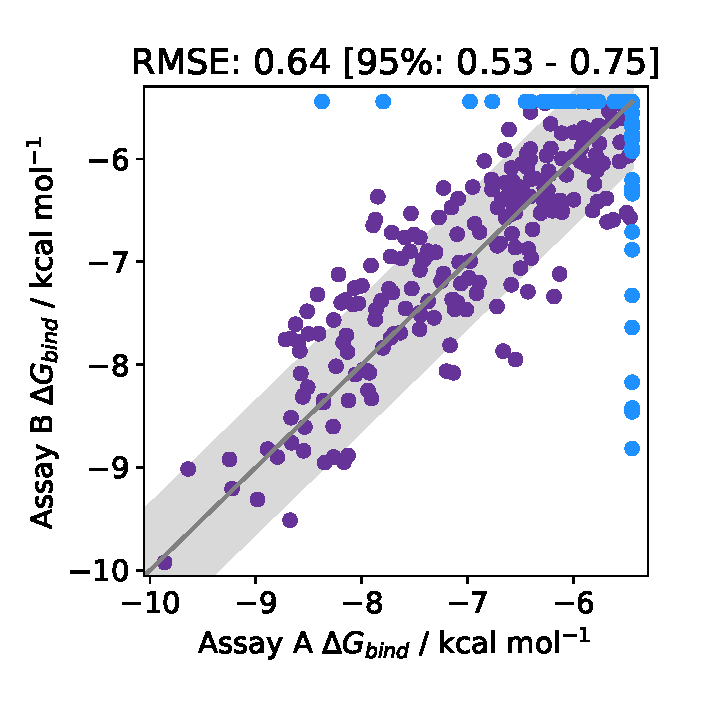
\includegraphics[width=0.95\linewidth]{figures/reporting/moonshot-assays.pdf}
    \caption{\textbf{Experimental uncertainties can be on the order of 0.64 kcal mol$^{-1}$.} The binding affinity of 365 molecules assayed by two different methods for the open source COVID moonshot project\cite{achdout2020covid}. Molecules that were predicted to bind in one assay, but inactive (i.e. affinity lower than the assay limit) the other are shown in blue. The RMSE agreement between the methods, for both purple and blue data points is 0.64 kcal mol$^{-1}$. Data was collected from the PostEra website\cite{posteracovid} accessed 22/11/2020. The grey region indicates an assay variability of 0.64 kcal mol$^{-1}$.}
    \label{fig:expt_agreement}
\end{figure}





There are two main requirements to consider in order to ensure that the experimental data are representative of the physics-based binding free energy that is calculated from the simulations. First, the measured output should reflect or closely correlate with actual protein-ligand \emph{binding}. Second, the assay conditions and the protein-ligand system used in the simulation should match as closely as possible. The first point relates to choosing the appropriate type of experimental data to compare with. Ideally, these would be biophysical binding data such as $K_d$ determined from isothermal titration calorimetry (ITC) or surface plasmon resonance (SPR). However, this type of data is often only available for a small number of compounds in drug discovery projects (and the related literature), typically for a few representatives per series. In addition, ITC data are often only available for a narrow dynamic range.~\cite{wiseman_rapid_1989,chodera_entropyenthalpy_2013} Since having a sufficiently large data set with a large dynamic range is also very important (see below), it may often be necessary to use data from functional assays (e.g., IC$_{50}$ from a biochemical assay) instead. For this assay, correlation with a biophysical readout should be checked before using the system as a benchmark data set.\cite{kalliokoski_comparability_2013}

With regards to matching simulation and binding assay, as mentioned above, it is important to have detailed knowledge of the assay conditions available; e.g., salt concentrations and co-factors. This information is needed for setting up a simulation model that closely matches the experimental conditions (see Section \ref{sec:prep}). Generally, salt concentration should match experimental assay conditions to capture screening effects, though sometimes salt \emph{identity} may be varied because of force field limitations. For a benchmark set, experimental data with assay conditions involving many co-factors or multiple protein partners should be avoided. In addition, one should check which protein construct was used in the structural studies compared to the assay (see Section \ref{sec:struct_data}). These should match as closely as possible. 

Finally, a dataset used for benchmarking of free energy calculations needs to be suitable to draw robust conclusions on the success of the methods ideally by both accuracy and correlation statistics. Whether a dataset is suitable depends on the number of data points in the set, the experimental dynamic range and the experimental uncertainty. 

Quantifying the experimental uncertainty is necessary for understanding the upper-limit of feasible accuracy for a model.~\cite{brown2009healthy} Understanding this is both useful for fair comparison between methods, and for conveying the reliability of a model to medicinal chemists~\cite{griffen2020chemists}. Building predictive models becomes more difficult with (a) a small experimental dynamic range and (b) large experimental uncertainties. It is useful to understand the upper limit of success a computational method can have for a set of experimental results;
%
\begin{equation}\label{eqn:r2max}
    R^2_{\mathrm{max}} = 1 - \left(\frac{\sigma(\mathrm{measurement\   error})}{\sigma({\mathrm{affinity}})}\right) ^2,
\end{equation}
%
where $R^2_{\mathrm{max}}$ is the highest achievable $R^2$ for a dataset with a standard deviation of affinities ($\sigma(affinity)$) and an experimental uncertainty of  $\sigma\mathrm{(measurement\ error)}$\cite{sheridan2020experimental}. This relation is illustrated in \ref{fig:r2max}.

For a typical experimental error of 0.64 kcal mol$^{-1}$ (see above) and a desired $R^2_{\mathrm{max}} = 0.9$, a standard deviation of affinities $\sigma(\mathrm{affinity}) = 2.02 $ kcal mol$^{-1}$ ($\approx$1.5 log units) is required. Assuming a uniform distribution of experimental affinities in the dataset, this corresponds to a required dynamic range of 7.01 kcal mol$^{-1}$ (e.g., from $-12$ to $-5$ kcal mol$^{-1}$) or $\approx$ 5 log units (e.g., from 1 nM to 100 $\mu$M). This dynamic range and the associated standard deviation of affinities also allow to differentiate typical free energy methods from a trivial affinity prediction model where all predicted affinities $\Delta G_{\text{pred}}^i$ are equal to the mean experimental affinity $\sum_{i=1}^{N} \Delta G_{\text{exp}}^i$. Note that for such a model RMSE is equal to the standard deviation of the affinities $\sigma({\mathrm{affinity}})$, while there is no correlation between predicted and experimental affinities.



\begin{figure}
    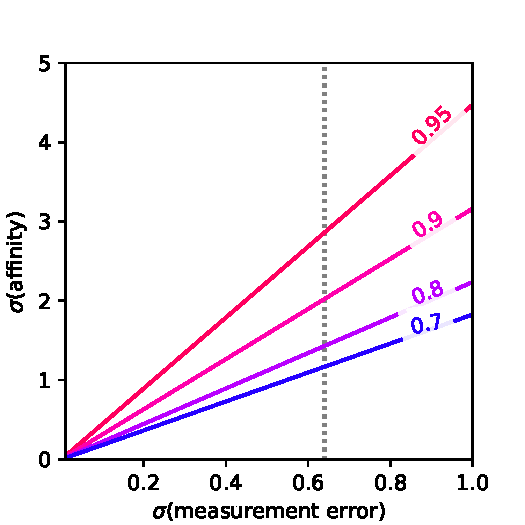
\includegraphics[width=0.95\linewidth]{figures/R2max.pdf}
    \caption{\textbf{The larger the experimental uncertainty, the larger the affinity range required for a given $R^2_{max}$}. Corresponding to Equation \ref{eqn:r2max}, the maximum achievable $R^2$ for a given dataset is limited by the range of affinities and the associated experimental uncertainty. The illustration assumes that $\sigma(measurement\ error)$ and $\sigma(affinity)$ are in the same units, with an experimental error of 0.64 kcal mol$^{-1}$ indicated.}
    \label{fig:r2max}
\end{figure}

In order to robustly evaluate statistics with small confidence intervals the dataset needs to be sufficiently large. Figure \ref{fig:N_CI} illustrates the dependence of the confidence interval obtained by bootstrapping for correlation statistics and accuracy statistics for simulated toy data. The "experimental" toy data were simulated using a uniform distribution with an affinity range of 7 kcal mol$^{-1}$ for the experimental toy data. This would be the recommended dynamic range for an experimental error of 0.64 kcal mol$^{-1}$ (see above). Predicted toy data were derived from the experimental toy data using a Gaussian distribution with standard deviation of $\sigma = 0.5$, 1 and 1.5 kcal mol$^{-1}$. While the absolute values that can be obtained for the correlation statistics are much affected by the dynamic range of the experimental data, the effect on the confidence intervals estimated via bootstrapping is relatively small.

Based on these simulations, we recommend a dataset size of 25 to 50 ligands. For a dataset size of 50, it is possible to distinguish between all three toy methods reliably in terms of RMSE. For an affinity prediction method with Gaussian error $\sigma = 1.0$ kcal mol$^{-1}$ this would yield the following estimated statistics: Kendall $\tau = 0.72_{0.62}^{0.80}$ and RMSE $= 1.0_{0.81}^{1.18}$ kcal mol$^{-1}$. Note that for relative calculations, a smaller number of ligands could be sufficient since multiple edges are typically evaluated for each ligand. On the other hand, for relative calculations, the experimental error for the relative free energies are larger because experimental errors for both ligands add up. 

\begin{figure}
    \centering
    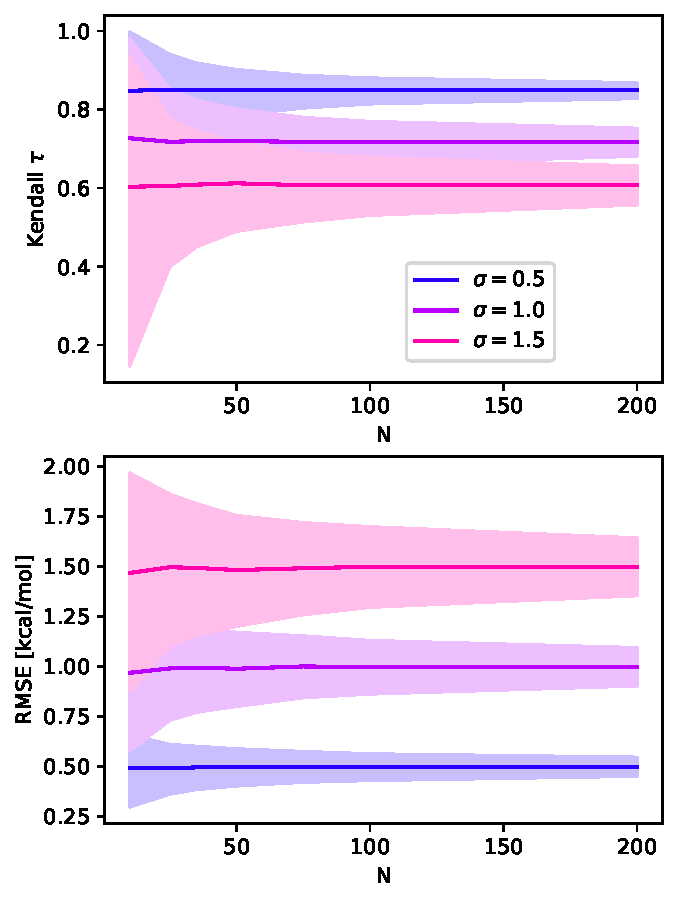
\includegraphics[width=0.95\linewidth]{figures/N-CI.pdf}
    \caption{\textbf{The larger the dataset, the smaller the uncertainty in the performance statistics}. Kendall $\tau$ and RMSE were evaluated for 1,000 toy datasets for a given size of the dataset $N$. The experimental data were simulated from a uniform distribution over the interval [-12:-5] and the predicted affinities were simulated from the experimental toy data using a Gaussian distribution with different standard deviation $\sigma$. The statistic was evaluated for the whole dataset and 95\% confidence intervals were estimated via bootstrapping. These were then averaged over all 1,000 toy datasets.}
    \label{fig:N_CI}
\end{figure}

As stated before, in practice it is challenging to find datasets that meet these criteria for dynamic range and number of ligands. We therefore currently recommend to annotate benchmark datasets according to these criteria to make challenges and limitations visible.

 
%%%%%%%%%%%%%%%%%%%%%%%%%%%%%%%%%%%%%%%%%%%%%%%%%%%%%%%%%%%%
%        Simulation setup and running simulations          %
%%%%%%%%%%%%%%%%%%%%%%%%%%%%%%%%%%%%%%%%%%%%%%%%%%%%%%%%%%%%
\section{How to best set up and run benchmark free energy simulations}
%%%%%%%%%%%%%%%%%%%%%%%%%%%%%%%%%%%%%%%%%%%%%%%%%%%%%%%%%%%%

%-----------------------------------------------------------
\subsection{Structure preparation}
\label{sec:prep}
%-----------------------------------------------------------

\begin{figure*}
    \centering
    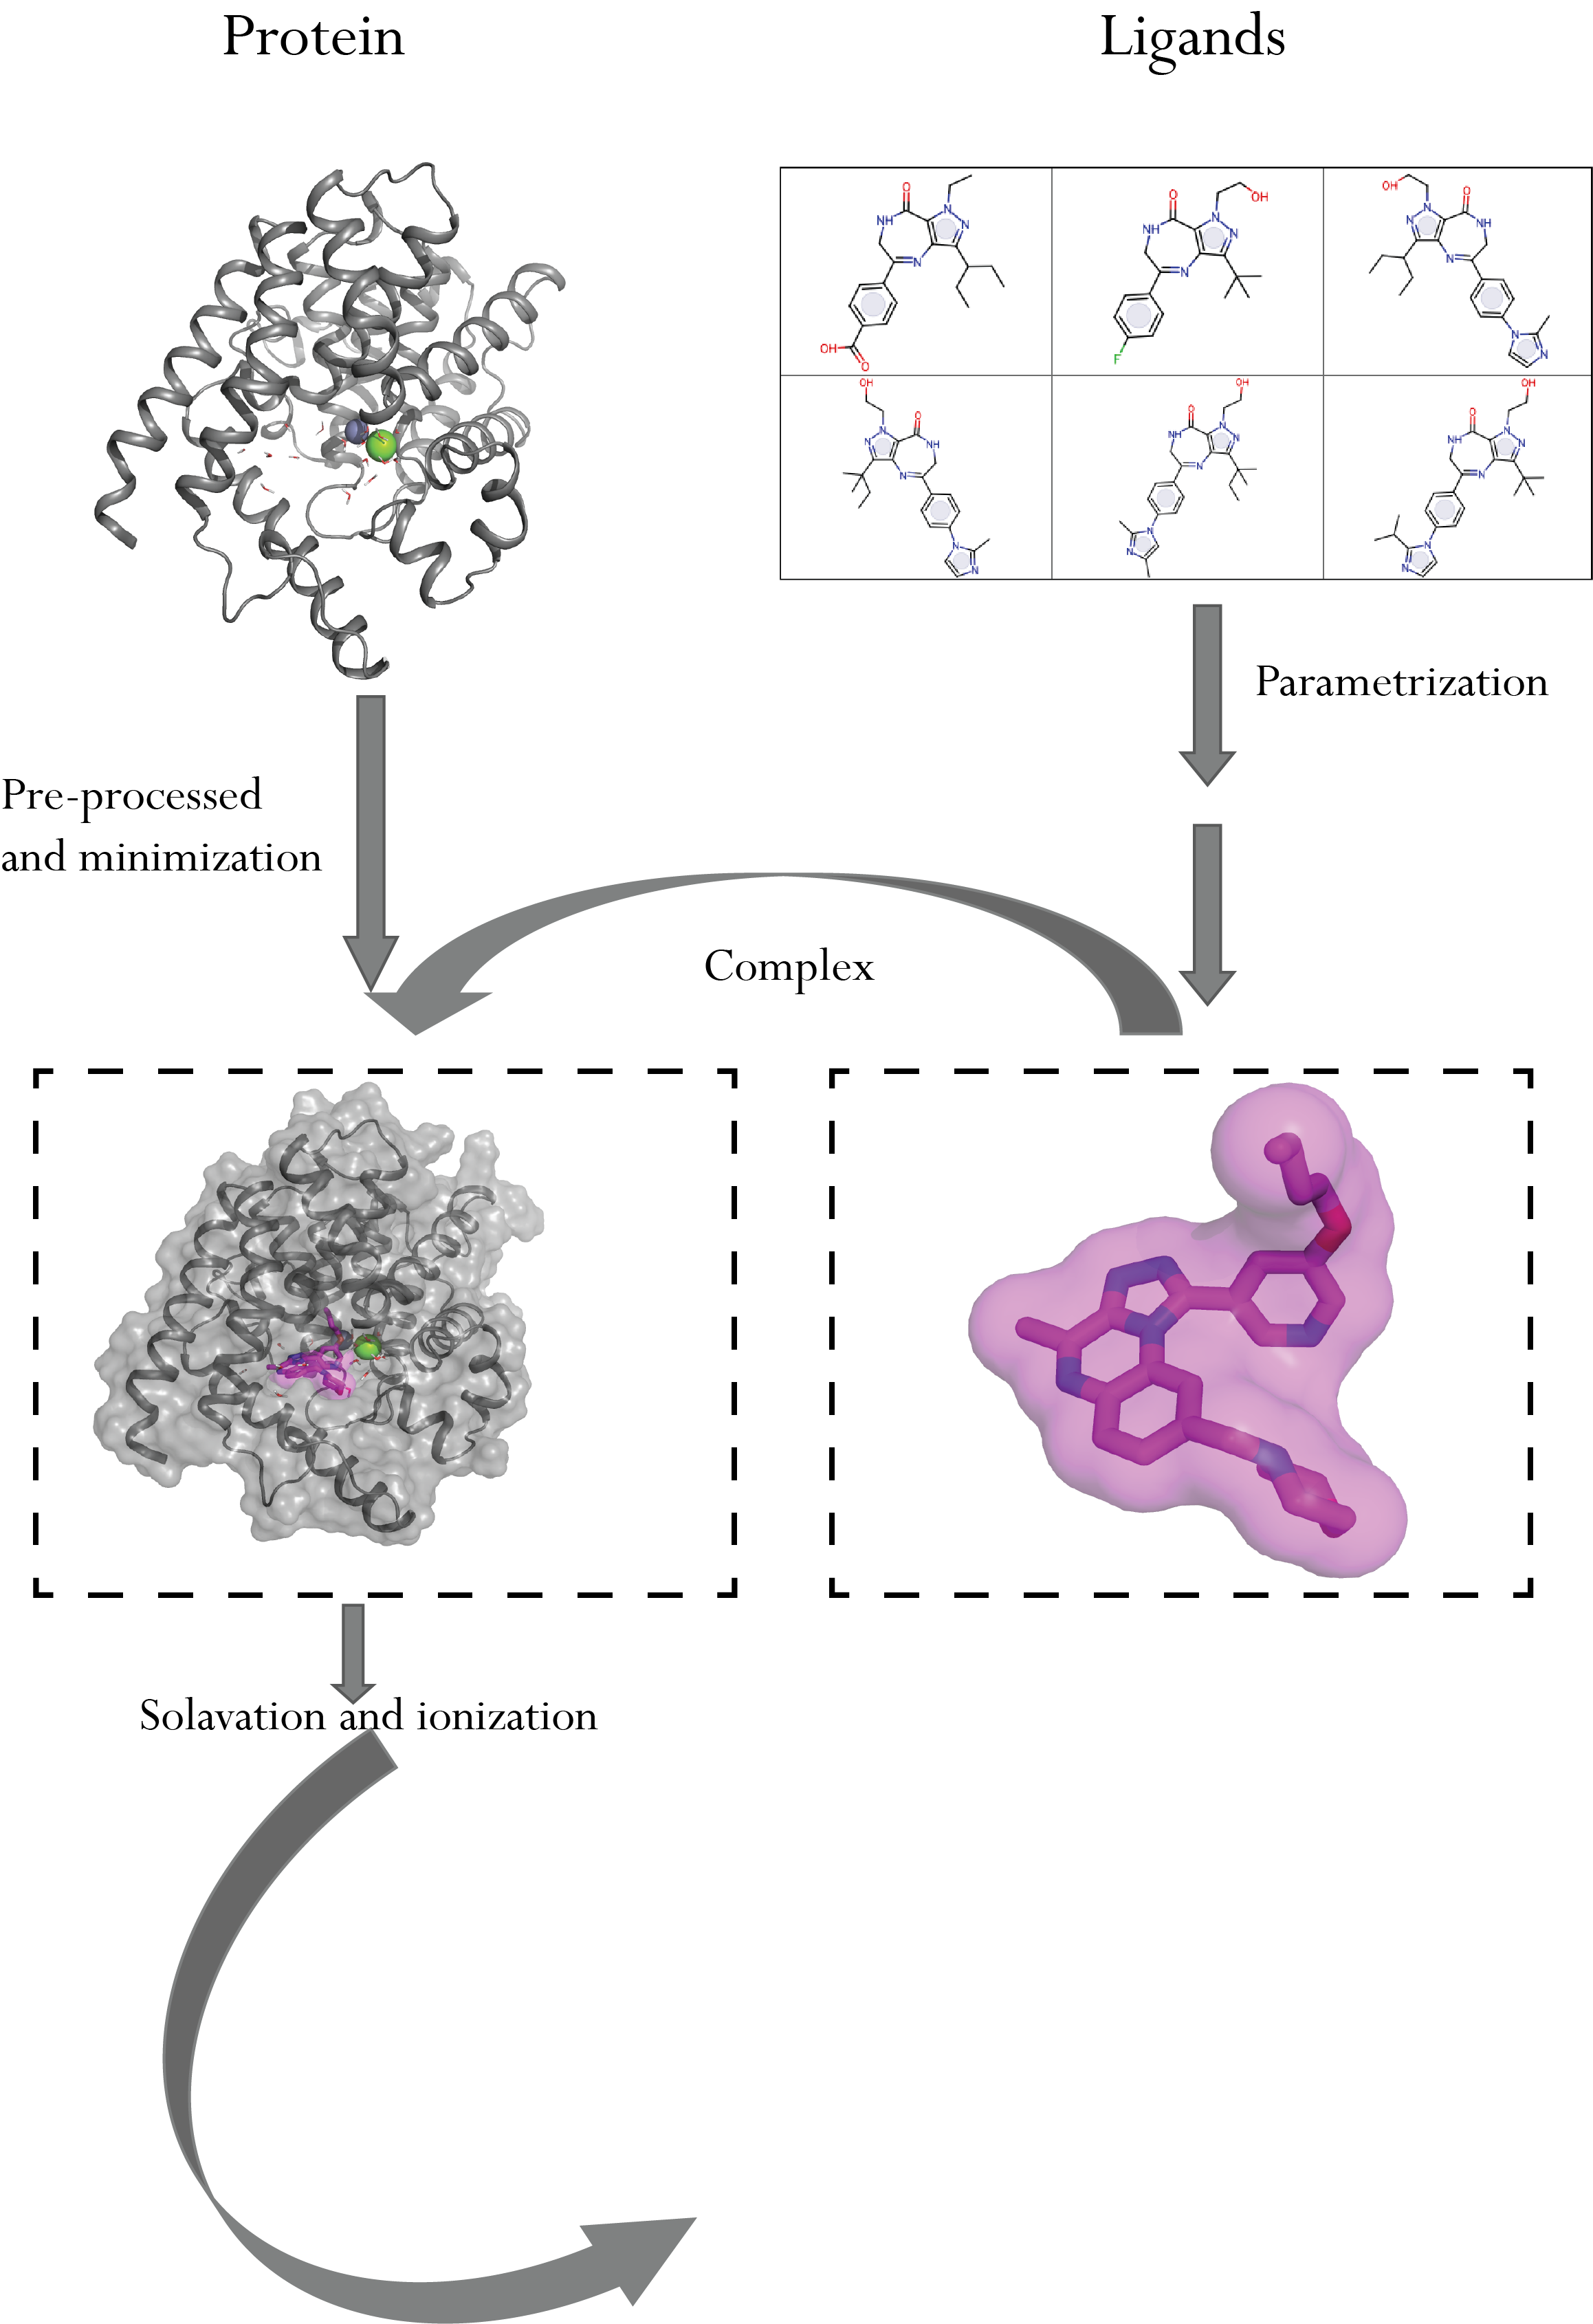
\includegraphics[width=.6\textwidth]{system_preparation.png}
    \caption{Outline of the system preparation steps.}
    \label{fig:system_preparation}
\end{figure*}

Starting with an experimental crystal structure, often an X-ray structure for the protein or protein-ligand complex, the most error-prone stage of protein preparation is the translation from an experimental result into a simulation model: inferring missing atoms and making choices about which X-ray components to include. Having chosen the crystal lattice monomer based on the criteria in the above section, you may wish to remove some domains of the structure if they are large and unlikely to affect the biological activities of interest. The truncation of the system needs to be assessed carefully as it has been shown in some cases, such as the dimeric form of PDE2 and the presence of cyclin with CDK2, that a more authentic representation of the system was beneficial for stability during simulations and improved free energy calculations. By decreasing the size of the overall simulation system while keeping the biological activity, large computational efficiencies can be realized with potentially minimal impact on results. Datasets for benchmarking may be run many times so this efficiency will be meaningful. 
%Working with cryo-EM structures can require an extra step. Even though we can find cryo-EM structures with a resolution around 3 Å, many are still commonly produced in the range of 4 to 10 Å, and in maps with these resolutions it can be difficult to predict side chain positions. Such low-resolution structures may not be appropriate for free energy calculations, better quality cryo-EM may be usable but require using classical MD for extra stability checks and system optimization prior to free energy calculations.

In addition to the protein itself, the subsystem you carry forward from the X-ray structure into simulation may have other components: ligand, cofactors, structural waters, other ligands (if you are simulating a multimer), post-translational modifications (PTMs), and excipients. The cofactors should be deliberately included or excluded based on their role in the biological activity being modeled, removing a cofactor from its cavity might cause unexpected movements or collapse of the cavity during the simulations. To avoid this, a careful equilibration and solvation of that pocket might be needed. All structural waters close to the protein should be included: in principle the MD sampling could allow waters to arrange in equilibrium positions, but experimental and theoretical work has shown that the timescales for this can be impractically long. Also, internal structural waters even very distal from the active site are integral to the protein structure, and omitting them can adversely affect the protein dynamics. Generally, we recommend to exclude excipients (often specific to the crystallization media and not present in the assay). PTMs require a judgement call: surface-exposed and distal from the active site they can often be safely excluded, for example glycosylations which could otherwise greatly increase the size of the calculation. This again can save on the overall system size and parameterization difficulties. PTMs proximal to the active site or known to be directly implicated in activity should be retained. Ligands other than that in the active site are again a judgement call: in principal retaining them is only necessary if there is biological cooperativity in the biological assay; in practice this is often not known so in general they should be kept if possible. 

We will consider the protein preparation first. The protein itself frequently has missing parts due to the lack of supporting data (electron density) from the X-ray experiment, for example N-terminal and C-terminal residues, mobile loops (e.g. the activation loop in kinases), and residue sidechains. Also, there can be extra parts as "alternate locations" (AltLocs): residue sidechains, or occasionally entire residues or the ligand, for which the experimental density supports more than one distinct orientation in a single x-ray structure solution. For the simulation, the protein must have all the atoms provided for every residue modeled. Missing residue sidechains should always be modeled in, assigning them the most preferred rotamer given the local environment. If N- and C-terminal sequence is missing due to disorder (lack of electron density), this is actually an experimental basis for omitting them from the model, but the truncated N- and C-termini should be "capped" by neutral termini, usually an acetate (ACE) cap on the N-terminus and an N-methyl (NME) cap on the C-terminus to mimic the peptide backbone out to the carbon-alpha. Of course, one must be careful not to cap the charged protein termini which are properly resolved in the X-ray: these can be critical for function and/or structure. This "capping" tactic can also treat the termini of "gaps": regions of missing residues over the span of the peptide chain, usually missing loop regions (again due to lack of experimental density). While capping the ends of a loop instead of modeling the whole loop may be acceptable for MD runs of relatively short duration, over longer simulations there is a risk of having the protein around the capped ends of the missing loop gradually lose its structure. Even if a loop is unstructured (and therefore missing in the x-ray structure), it is still holding the ends together. Strategic use of a distance restraints can mitigate this liability. Another possibility for missing loops is to close the ends with a short modeled loop of glycines of sufficient size to link the termini without introducing strain, but not necessarily of the full length of the missing loop. There are several reasons why this can be desirable. If the missing loop is particularly large (for instance >15 or 20 amino acids) accurately modeling its conformation could be challenging and introduce more uncertainty and instability to MD simulations. Furthermore, if the missing loop is distal from the binding site and not expected to affect protein ligand interactions, the replacement only needs to provide a role to stabilize the termini and with the advantage of avoiding the use of restraints. However, a good quality modeling of the missing loop would be preferable. With AltLocs, we have the opposite problem: the experimental data tells us that the fragment possibly exists in two (or more) mutually exclusive orientations experimentally, but we must choose one for our model. Again, this is a judgement call depending on where the AltLoc occurs relative to the active site: distal from the active site, the choice may be less critical; proximal requires more careful consideration. Higher occupancy for one of the AltLocs would be a reason to choose that one for the model.

Once the above issues have been resolved, there remains one more round of decision-making: sidechain flips for HIS, ASN, and GLN, and finally protonation states. Protein X-ray experiments cannot resolve the positions of hydrogens, and as importantly they cannot distinguish between different first-row elements O, N, and C: they all look the same. This means that even with good electron density the sidechain orientations of ASN and GLN can have either orientation, swapping O and N positions, and thus interchanging H-bond donors and acceptors. The two possible orientation of HIS sidechains effectively interchange N and C positions in the ring, though it is actually a ring flip. Surface exposed, these different orientations may be of little consequence, but in the interior of the protein, proximal to the active site, or especially interacting with the ligand, this can be very important. In principle these orientations can be sampled over the course of the MD run but only if the trajectory is long enough for the sampling scheme to allow it. Considering that these orientations are experimentally ambiguous, it is a matter of judgement at setup time of whether these sidechains should be reoriented to make a more chemically reasonable model. Historically, the rather long list of tasks above would be done by hand; these days there are a number of tools available to automate many of them... but caveat emptor!

Protonation of the protein model is generally straightforward with one key exception: the ionization state of ionizable sidechains, most particularly ASP and GLU. Active site catalytic CYS is another case requiring care, and occasionally LYS can be deprotonated in some circumstances. The two main determining factors are the pH of the biological milieu and the microscopic environment around the ionizable sidechain. In general, the ionization state of each residue is chosen parametrically during the setup of the protein and remains constant over the course of the simulation, even if the microenvironment changes. 
%There are some "constant pH" MD methods available which down the road could offer a more palatable alternative once they have been integrated with free energy methods. 
Note that a formal charge on the bound ligand can also affect the ionization state of nearby protein residues; this can be particularly problematic when the ligand charge alchemically changes over the course of a relative free energy calculation.

In the preparation of the ligand for simulation it is important to verify that the chemical structure is correct. While this is less of a problem for structures generated from small-molecule sources, historically it has been a frequent problem for ligands taken from protein-ligand X-ray structures. Once the underlying chemical structure, including bond orders and stereochemistry, is correct, the key issues are the  tautomer and ionization states. As with the ionizable protein residue discussed above, the main factors are the macroscopic pKa of the ligand (for ionization states), the intrinsic relative stability of different tautomer states, and the perturbing effects of the active site microenvironment of the bound ligand. Compounding the complexity is if the unbound ligand (used as a reference state) would have a different tautomer/ionization state. These need to be carefully examined at setup to make sure there is complementarity between the protein and ligand independently of the alchemical change between ligands, and then to flag and resolve alchemical conversions between inconsistent states of the protein.

Once protein and ligand have been prepared, the complex is assembled and solvated in water, or embedded in membrane if the protein belongs to a membrane protein family. In this last case you should use an appropriate equilibrated membrane that matches experimental criteria of thickness and area per lipid as well as the appropriate counter ions. Once the system box is constructed the step involves neutralizing the net charge on the protein-ligand complex, but beyond this a higher concentration of salt (usually sodium chloride) is often warranted to mimic the biological milieu being modeled; most assays are run in a significant salt concentration (100 to 150 mM) to emulate biological environments. The salt concentration can strongly affect experimental binding affinities, particularly with highly polar active sites.

Once the above decisions have been made and the complete simulation system has been set up, it is important to let it relax and equilibrate at simulation temperature and pressure, which should mimic the assay conditions.

%-----------------------------------------------------------
\subsection{There are specific challenges for alchemical free energy calculations during setup}
\label{sec:alchemical_prep}
%-----------------------------------------------------------

There are an abundance of details that must be considered during the set up of any simulation and in particular for alchemical free energy calculations. The two main differences between an alchemical free energy simulation setup and a conventional MD simulation are: an alchemical perturbation of the small molecules needs to be created, and the assumptions that are made with respect to the environment at the two endstates. In the following we will address all essential choices that need to be made for the setup. For a very detailed introduction to best practices for alchemical free energy calculations and a much broader discussion on choices for their setup please refer to the best practices guide~\cite{meyBestPracticesAlchemical2020}. 

\subsubsection{Should I run an absolute or relative free energy calculation?}
There are two possible ways in which to run alchemical free energy calculations, which both provide free energies of binding, but will require different routes for their setup. \textit{Relative} free energy calculations provide free energies of binding with respect to a reference ligand, meaning that all compounds that are to be assessed for their binding affinity should share a similar scaffold. Whereas \textit{absolute} free energies of binding can be used for a dataset of ligands that do not share any commonalities as the reference state for the free energy of binding is the standard state. This is probably the easiest deciding factor in terms of what kind of calculation to run. If the particular benchmark dataset contains ligands that form a congeneric series then a relative calculation is likely a better choice. Of course congeneric ligand series can be assessed using absolute free energy calculations, or it may be of interest to compare relative to absolute calculations for a given benchmark dataset. 


\subsubsection{Alchemical pathway}

\paragraph{Choices in topology}
The choice of topology, may be dictated by the simulation software of choice as not all common MD codes implement all topologies. The topology refers to the way in which a molecule A is changed to molecule B. Selecting either a dual or single topology approach is acceptable, unless performance of different topologies is assessed across the benchmark datasets. For more details on the different topology choices and implementations please refer to Mey et al.~\cite{meyBestPracticesAlchemical2020} al.~\cite{meyBestPracticesAlchemical2020}.
\paragraph{Choices around $\lambda$}
In order to connect the initial and final state of the alchemical free energy calculation an alchemical pathway must be chosen. This pathway is regulated by a variable $\vec{\lambda}$, which at $\vec{\lambda}=0$ represents molecule A and at $\vec{\lambda}=1$ molecule B. As free energy is a state function, the computed free energy is in principle independent on the pathway, but different choices in pathway can make the problem computationally more or less tractable. The simplest way to switch between molecule A and B is using a linear switching function for the potential energy of the form:
\begin{equation}
U(\vec{q},\vec{\lambda}) = \vec{\lambda} U_0(\vec{q}) + (1-\vec{\lambda})U_1(\vec{q}),
\end{equation}
where $U$ is the potential energy $\vec{q}$, is the set of positions and $\vec{\lambda}$ the switching parameter. Considerable care needs to be taken in selecting the switching function and spacing of so-called $\lambda$-windows. Common choices are, how many $\lambda$-windows should be used? What functional form should my switching function take? The concept of \textit{difficult} and \textit{easy} transformation is more and more explored, but currently heuristics based on phase space overlap between neighboring $\lambda$-windows is the best way to assess how many windows should be simulated. This can for example be done by looking at the off-diagonals of an overlap matrix~\cite{klimovich_guidelines_2015,kuhn_assessment_2020}. Furthermore, the choice of simulation protocol will influence what switching function and how many $\lambda$-windows should be used. 
%- Alchemical protocol  (Alchemical path, coupling function?), which can be any function, presumably monotonic, that at no stage leaves naked charges.
%- Number of lambda windows - compromise between computational expense and results
%- Spacing of lambda windows - mention trailblaze? But want reasonable exchange (if exchange is happening)


\subsubsection{Choice of Simulation protocol}
There are currently four common types of simulation protocols available, which are summarised in Fig.~\ref{fig:protocols}, these are: Fig.~\ref{fig:protocols} (A) independent replicas, (B) replica exchange, (C) Single replica, self adjusted mixture modelling and (D) non-equilibrium switching. Particularly for (B) and (C) the choice of $\lambda$-spacing will be important, as in (B) it dictates the success of replicas exchanging between $\lambda$s and in (C), often tightly spaced replicas allow for a best exploration. Independent replicas are not necessarily recommended, but are still commonly implemented in software packages. 
\begin{figure}
    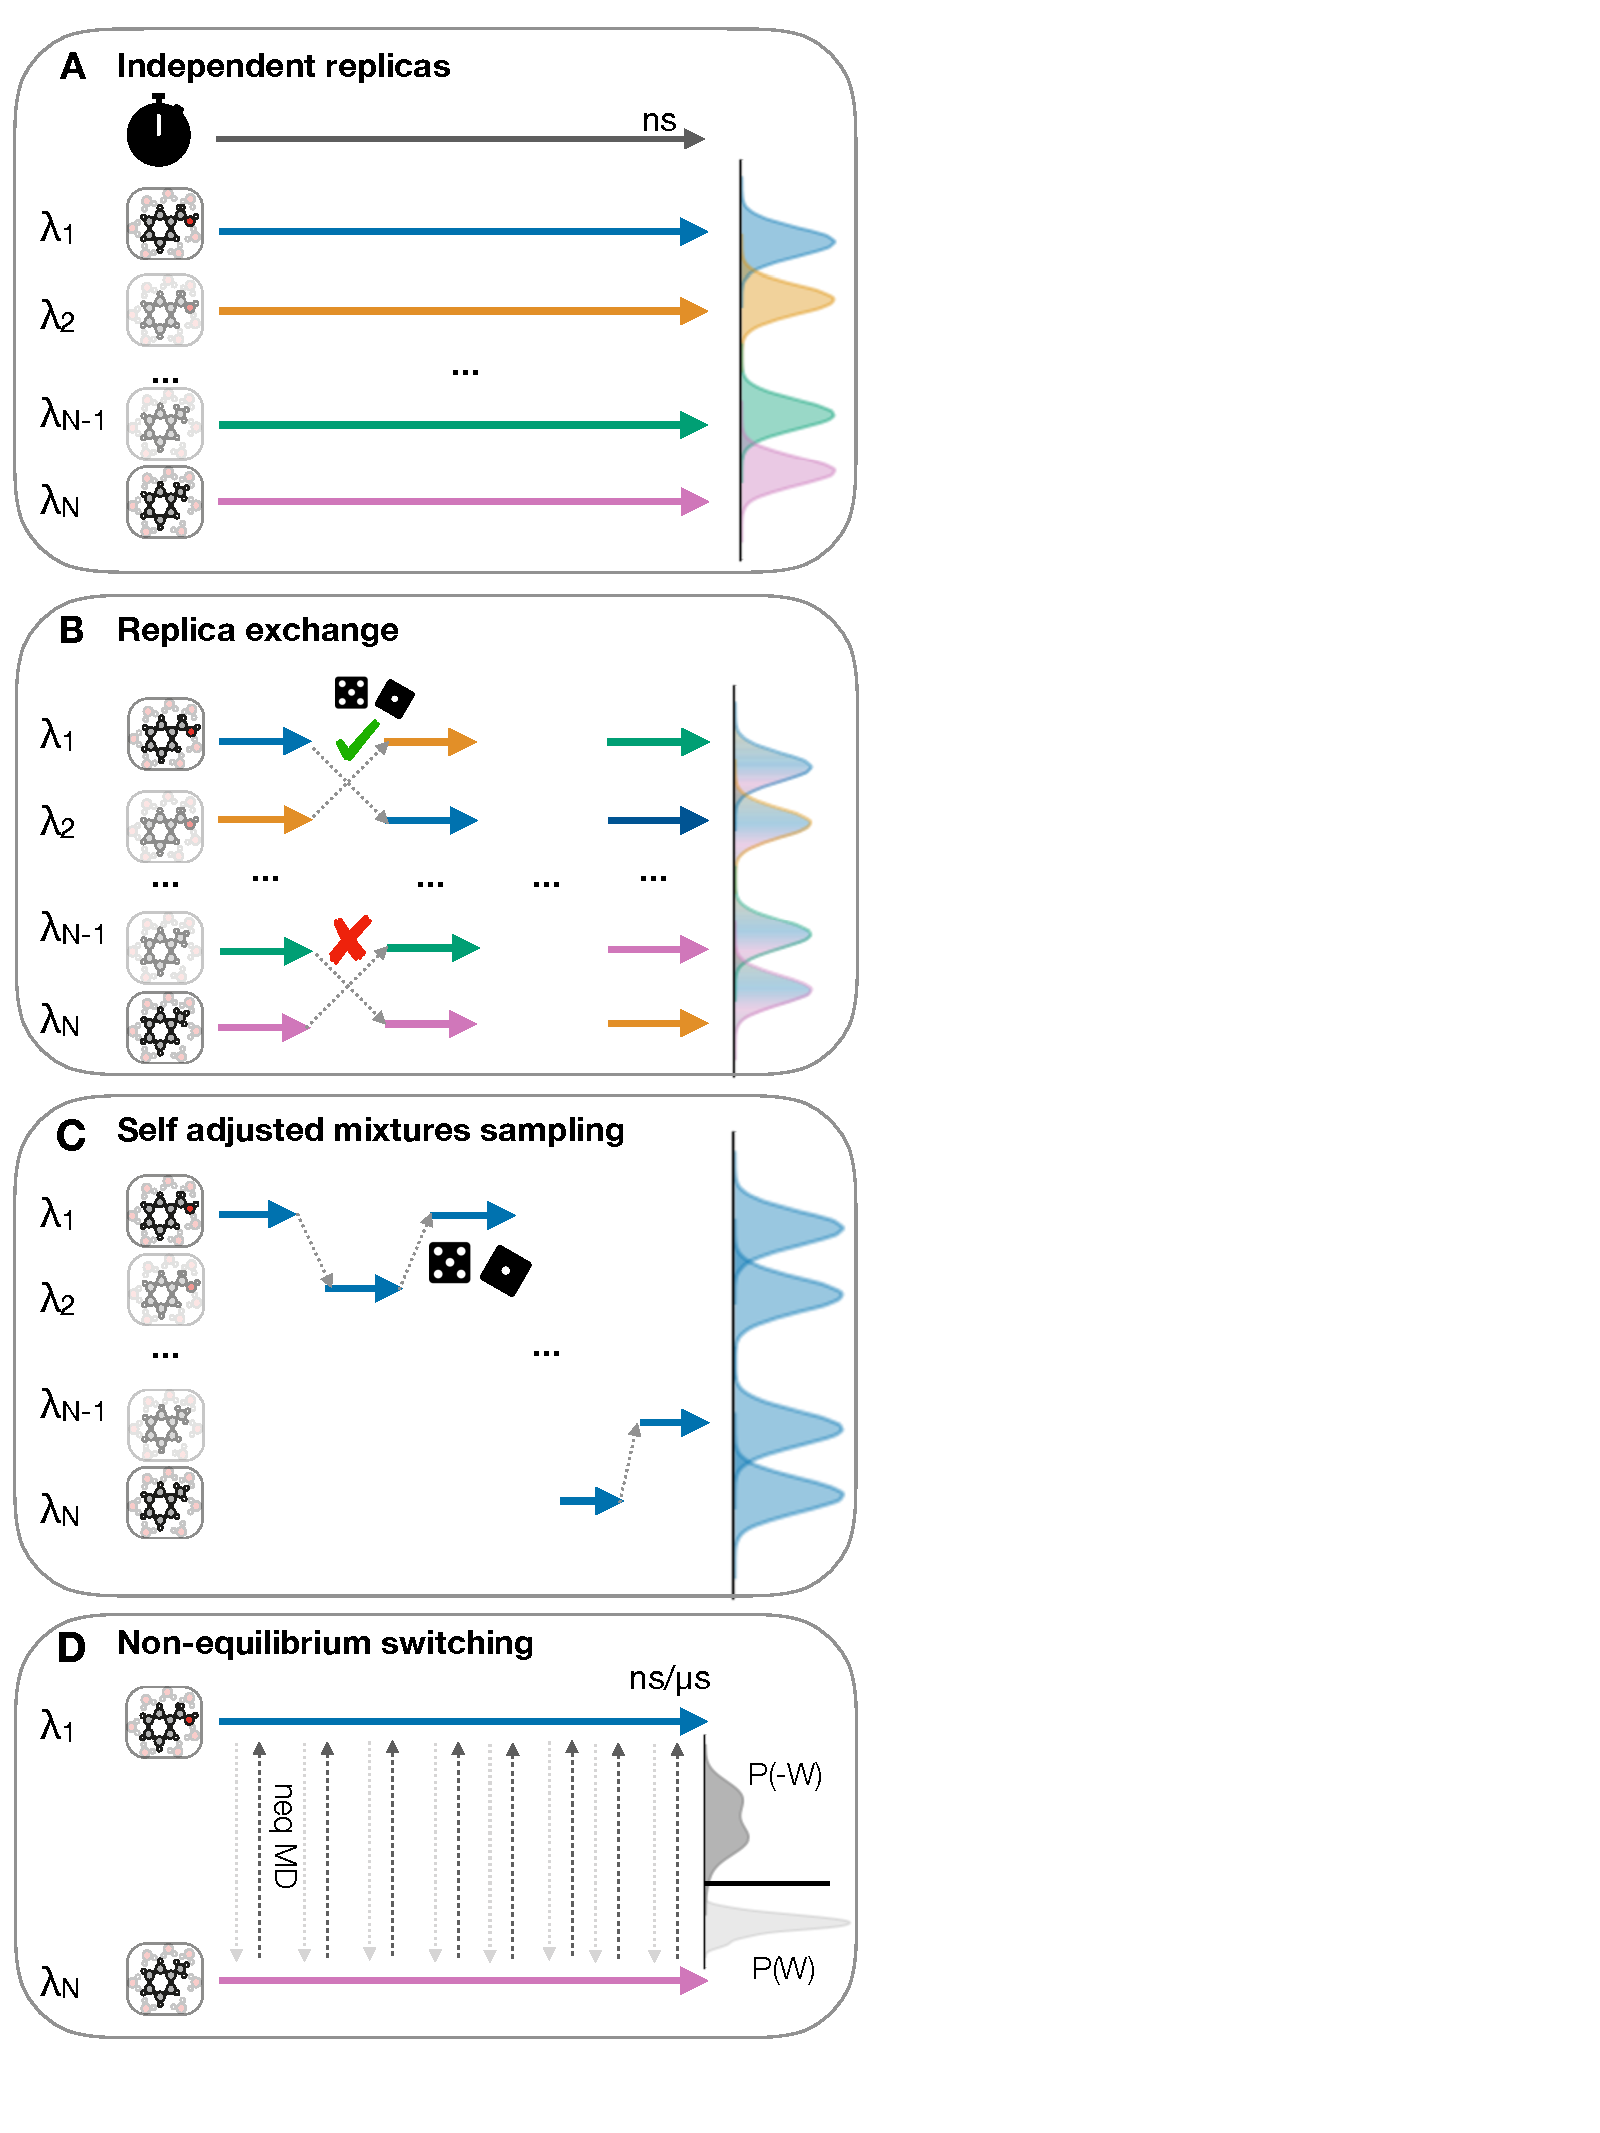
\includegraphics[width=0.95\linewidth]{figures/setup/protocol/Figure.pdf}
    \caption{\textbf{There are four simulations protocols available for generating samples and all $\vec{\lambda}$ states.} (A) Independent replicas run in parallel at different $\lambda$s as indicated by differently colored arrows, (B) Replica exchange attempts after short simulation for each replica (C) Self-adjusted mixture sampling with a single replica exploring all of $\lambda$, (D) Non-equilibrium methods with equilibrium end-state simulation and frequent non-equlibrium switching between endstates. The clock icon is indicating the flow of simulation time and the pair of dice indicate a Metropolis Hastings based trial move}
    \label{fig:protocols}
\end{figure}

\subsubsection{End-state environments}
When setting up a relative calculation it is important to be aware of the similarity of the 'end states', i.e. of the conformational, hydrational, and charge environment of ligand A and B. Many of these end-state issues can be addressed with infinite sampling, but this may be impractical and should be considered when planning perturbations. Issues can arise, if there are two distinct bound conformations (different binding modes) for ligand A and ligand B, it may be necessary to sample both binding modes, or extend the simulation time to allow for sufficient rearrangements. A similar issue that may be addressed with extended sampling times are scaffold changes that occur between ligand A and B. Different hydration patterns may also cause inaccuracies in computed binding free energies. The probably most difficult issue to address are changes in charge states that occur either between the two ligands or may even affect the protein depending on the type of ligand binding. 
%- Will the protein be in two distinct conformations when bound to the two ligands, significant active site rearrangement - theoretically fixable with infinite sampling
%- Will there be a conformational change in the structure of the ligand scaffold during the alchemical transformation (similar issue as above)  - again infinite sampling would fix this
%- Will both endstates have the same active site hydration pattern - again infinite sampling would fix this
%- Will a change in the ligand (charge possibly) result in a charge change in the protein - not fixable with infinite sampling (David: Charge change in protein could - theoretically - be also part of the alchemical transformation, no?)

\subsubsection{Perturbation maps for relative calculations}
In relative free energy calculations a network of perturbations between ligands can be constructed. The choice of which relative calculations is vast and can have a substantial effect on the accuracy of the results. The way in which different ligands are connected by relative alchemical calculations is called a perturbation map. In particular for benchmarking it would be vitally important to use the same type of perturbation maps for the same benchmark sets unless new methodologies on how to setup perturbations maps are tested. In this way each edge of the perturbation map will be the same and plots created during the analysis phase later will be comparable. The simplest way of connecting ligands is in a star shape, with each connected to a central crystal structure ligand, with the assumption that all ligands of the congeneric series will bind in the same binding mode as the available crystal -- which may even be confirmed by other crystals, see Fig.~\ref{fig:map} (A), there are different methods available for creating interconnected perturbation maps using LOMAP~\cite{liu_lead_2013} or Diffnet~\cite{xu_optimal_2019}, as well as some work towards assessing trade off in terms of what network structure will actually provide most reliable estimates with as little computational cost as possible~\cite{yang_optimal_2020}.

\begin{figure}
    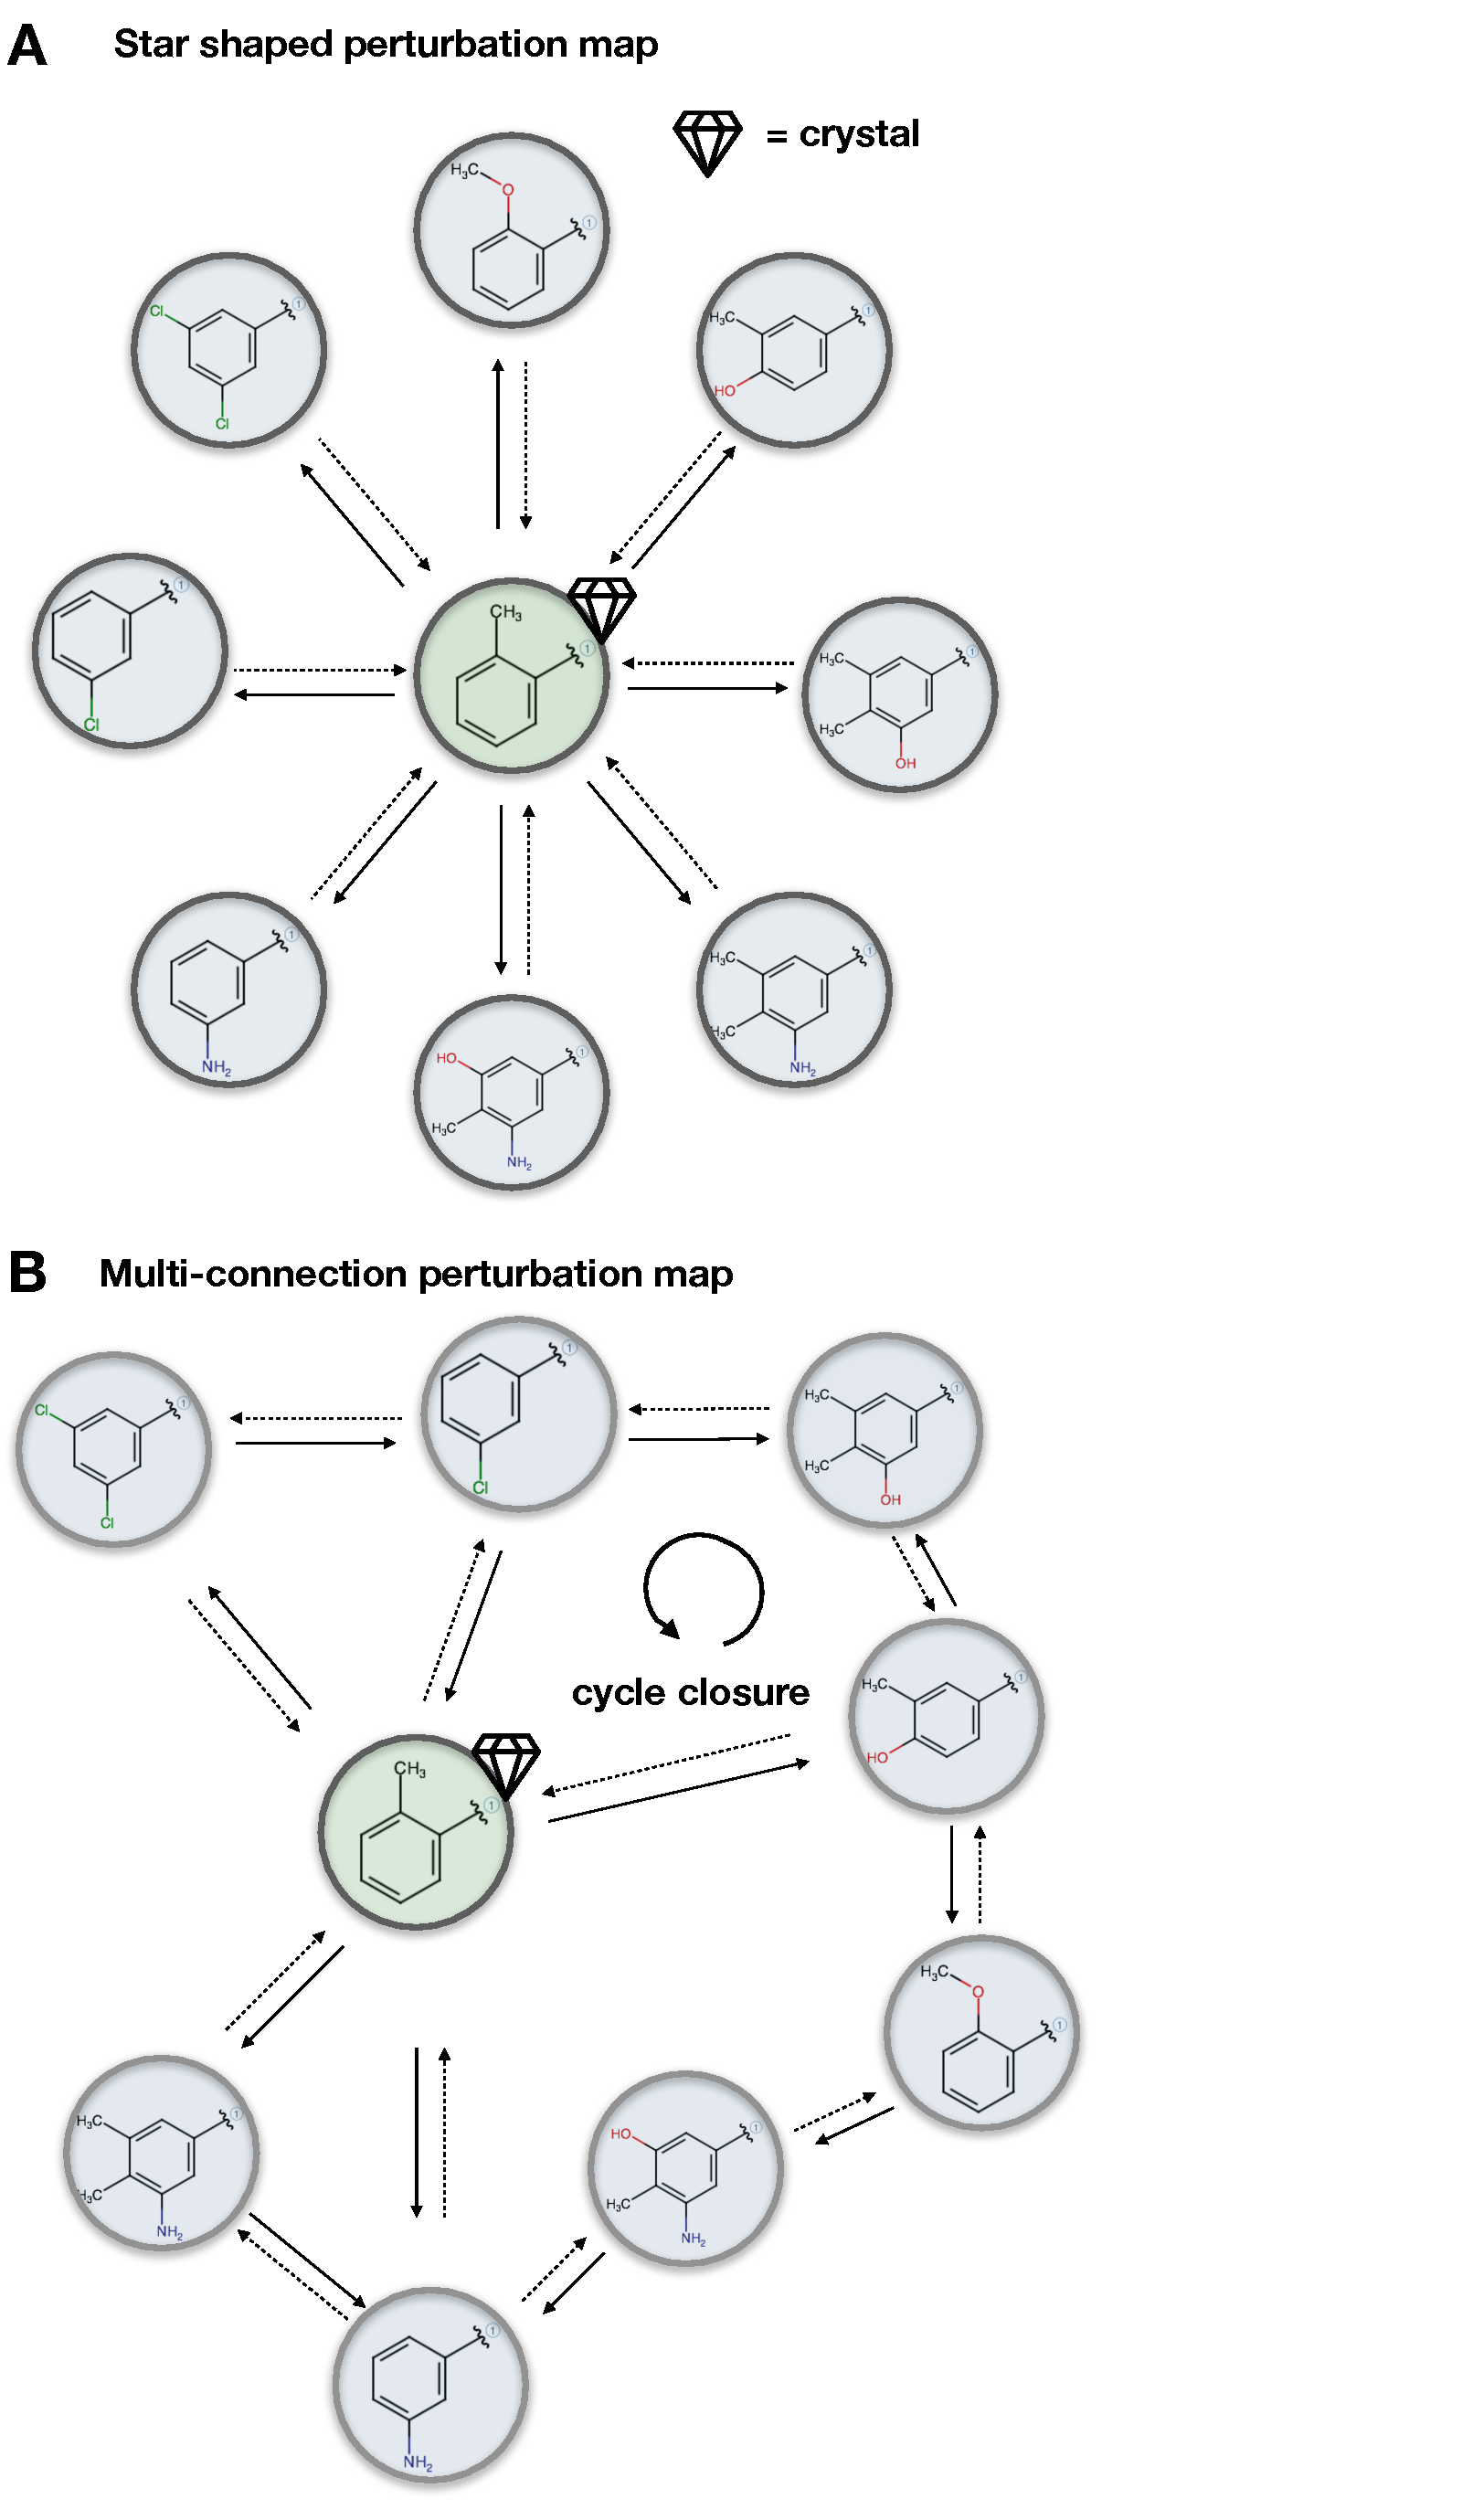
\includegraphics[width=0.95\linewidth]{figures/network.pdf}
    \caption{\textbf{Typically either star shaped perturbation maps or multi-connected perturbation maps are used in relative calculations} (A) The star map will have a central ligand, of which the crystal structure is known and all other ligands distributed in a star. (B) A multi-connected map introduces redundancies into the network, allows for larger perturbations through multiple connections and allows assessment of robustness of calculations. The diamond and green shading indicates the crystal structure.}
    \label{fig:map}
\end{figure}

- inclusion of intermediates
- MCS
- Ring breaking


%%%%%%%%%%%%%%%%%%%%%%%%%%%%%%%%%%%%%%%%%%%%%%%%%%%%%%%%%%%%
%                    Simulation analysis                   %
%%%%%%%%%%%%%%%%%%%%%%%%%%%%%%%%%%%%%%%%%%%%%%%%%%%%%%%%%%%%
\section{How to analyse benchmark free energy simulations properly}
\label{sec:analysis}
%%%%%%%%%%%%%%%%%%%%%%%%%%%%%%%%%%%%%%%%%%%%%%%%%%%%%%%%%%%%

%-----------------------------------------------------------
\subsection{Measuring the success of free energy calculations requires careful analysis}
%-----------------------------------------------------------

Reliable reporting and analysis of the success of calculations is vital for the validation and benchmarking of free energy methods as well as the dissemination of published results. This reporting and analysis falls into two major categories -- visualization of results, and statistical analysis. Here we make recommendations for both categories.

\subsubsection{Plots of free energy results should adhere to certain common standards}
\label{sec:plotting_results}
Figures plotting experimental vs. calculated results are a very useful way to gauge the success of a method or a set of calculations. We recommend several key steps to ensure these plots are valuable, communicate accurate information, and are informative and readable. Experimental values (on the x-axis) should be converted into the same units as the free energy results (on the y-axis), and axes should use the same scale. One common issue with plotting free energy results is that different scales are used on the different axes, which can change the appearance of the results, as illustrated in Figure~\ref{fig:plotting-basics}, where changes in the axis and ratios can make the data look more correlated.

\begin{figure}
    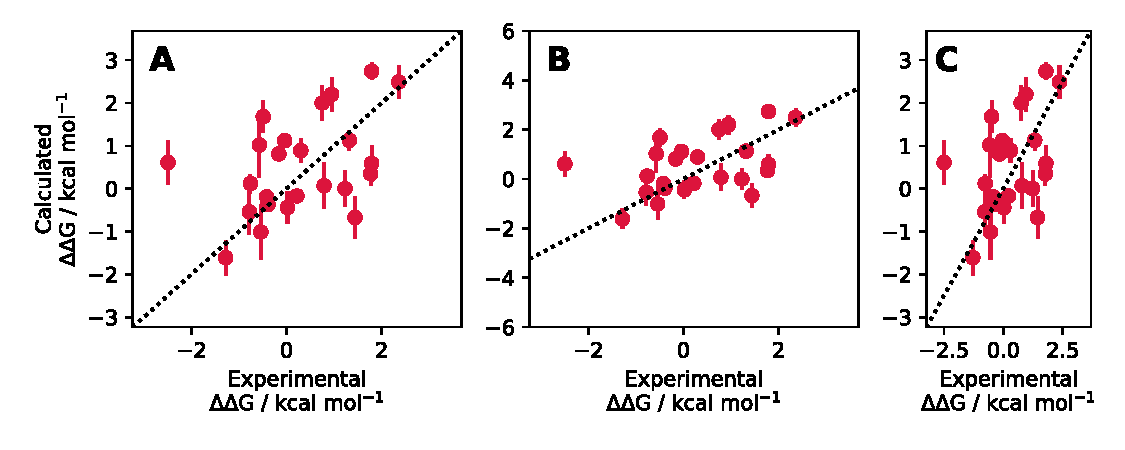
\includegraphics[width=0.95\linewidth]{figures/reporting/plotting-basics.pdf}
    \caption{\textbf{Changes to the plotting style can change the appearance of the data.} The above three figures illustrates the same toy data. A) shows the data correctly, with the same units (which are labelled) and scales on both axes. B) shows the same data, however the limits on the y-axis have been changed such that the scales is not consistent. C) is also not consistent, but this is due to the scale of the plot, rather than the limits.}
    \label{fig:plotting-basics}
\end{figure}

Error bars can be very helpful in understanding the uncertainty in the data -- both for calculated and experimental values, and thus both experimental and computational error bars should always be included in visualizations of the data. Different sources of error might be used to quantify this, whether an uncertainty directly from a free energy estimator, variance between repeats or a hysteresis-type analysis. If the experimental errors are not reported, the experimental error can be estimated (e.g. $0.64\,\mathrm{kcal\,mol^{-1}}$, see Section \ref{sec:affinities}) can be used. How the error bars have been calculated should be reported in the figure caption.


Additionally, experimental values which were not actually measured (e.g. values resulting from a measured $K_D$ value which only has experimental bounds, such as $> 5 \mu M$) should not be plotted or should be clearly indicated by different styles and symbols. These data should not be included in the accuracy or correlation statistics discussed in Section \ref{sec:statistical_analysis}, however confusion matrices and reporting sensitivity, specificity and precision can be useful for asserting a models' strength at classifying ligands as binders and non-binders, as demonstrated in \cite{hauserPredictingResistanceClinical2018}.

Finally, plots of results across various targets should typically show one figure per target. Differences in the success of free energy methods can vary widely between targets, and combining the data across targets onto a single plot can obscure actual performance on any given target. Additionally, when considering absolute free energies, the affinity ranges between targets may vary, which may result in analysis picking up the correlation between targets and their affinities, rather than the free energy methods ability to differentiate affinities for a particular target. One exception to this however may be if free energy calculations were being performed for selectivity analysis of similar proteins, whereby the targets are not independent parameters\cite{aldeghiPredictionsLigandSelectivity2017}.

\subsubsection{Consistent reporting of statistics, and understanding their limitations is vital for measuring success}
\label{sec:statistical_analysis}
Free energy calculations fall into two categories: absolute and relative. Depending on which type of result are being analyzed --- absolute or relative --- different statistics will be appropriate. Accuracy statistics, such as root mean squared error (RMSE) and mean unsigned errors (MUE) provide information as to how well the computational method recapitulates the experimental results, and allow for a 'best guess' as to how far the computation prediction of new ligands' affinities may be from experiment. Correlation statistics, such as $R^{2}$, Kendall tau ($\tau$) and Spearman's rank ($\rho$) indicate how well a method does at ordering the results, at identifying the best and worst ligand in a set, which in an everyday drug design application, where these models may be used to make purchasing decisions or for synthesis planning, may be a more useful metric than accuracy.



\begin{figure}
    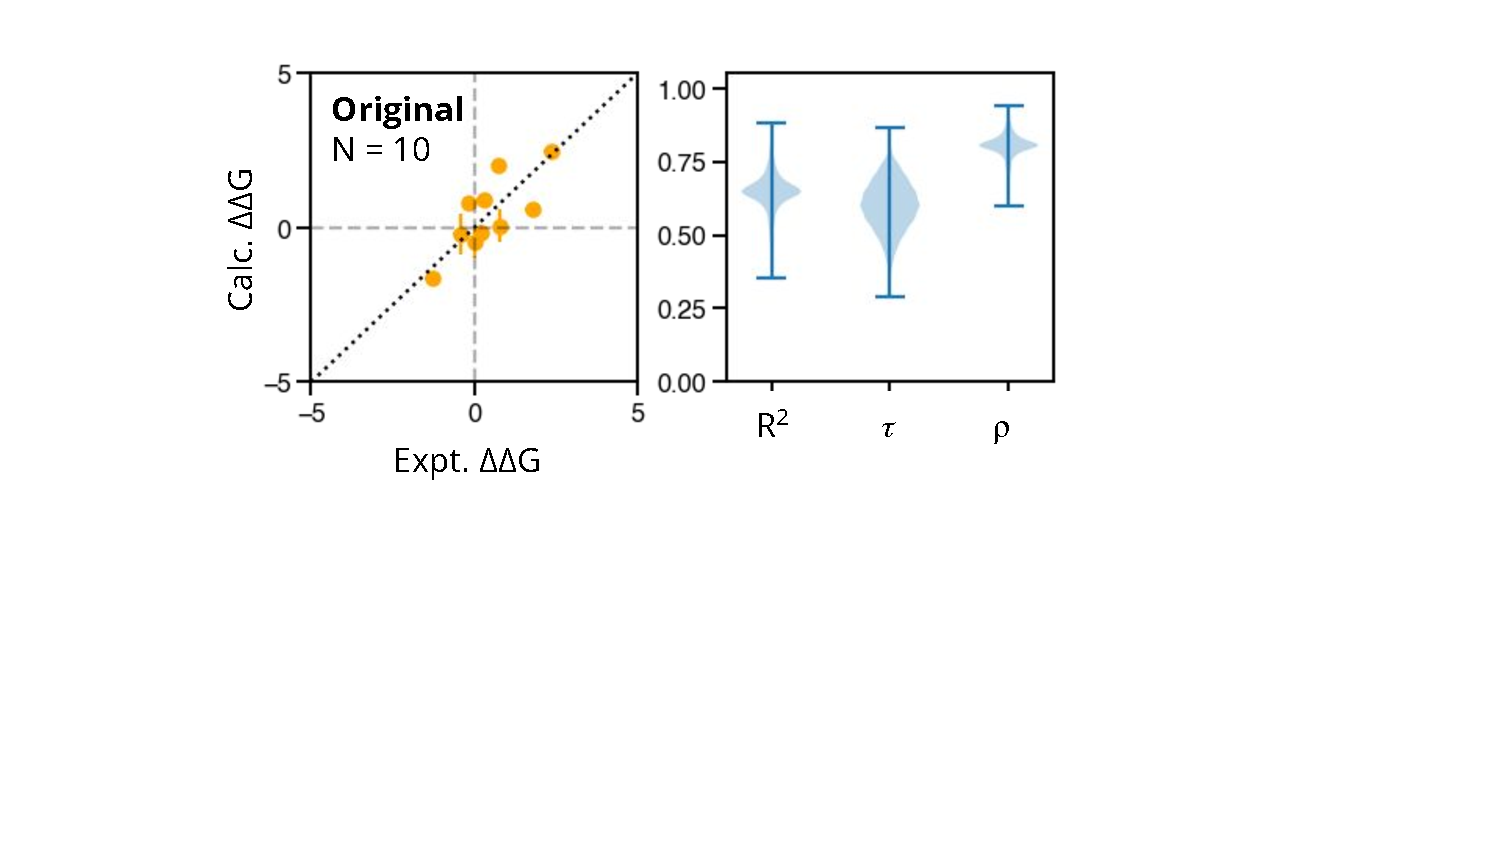
\includegraphics[width=0.95\linewidth]{figures/reporting/relativeissuesA.pdf}
    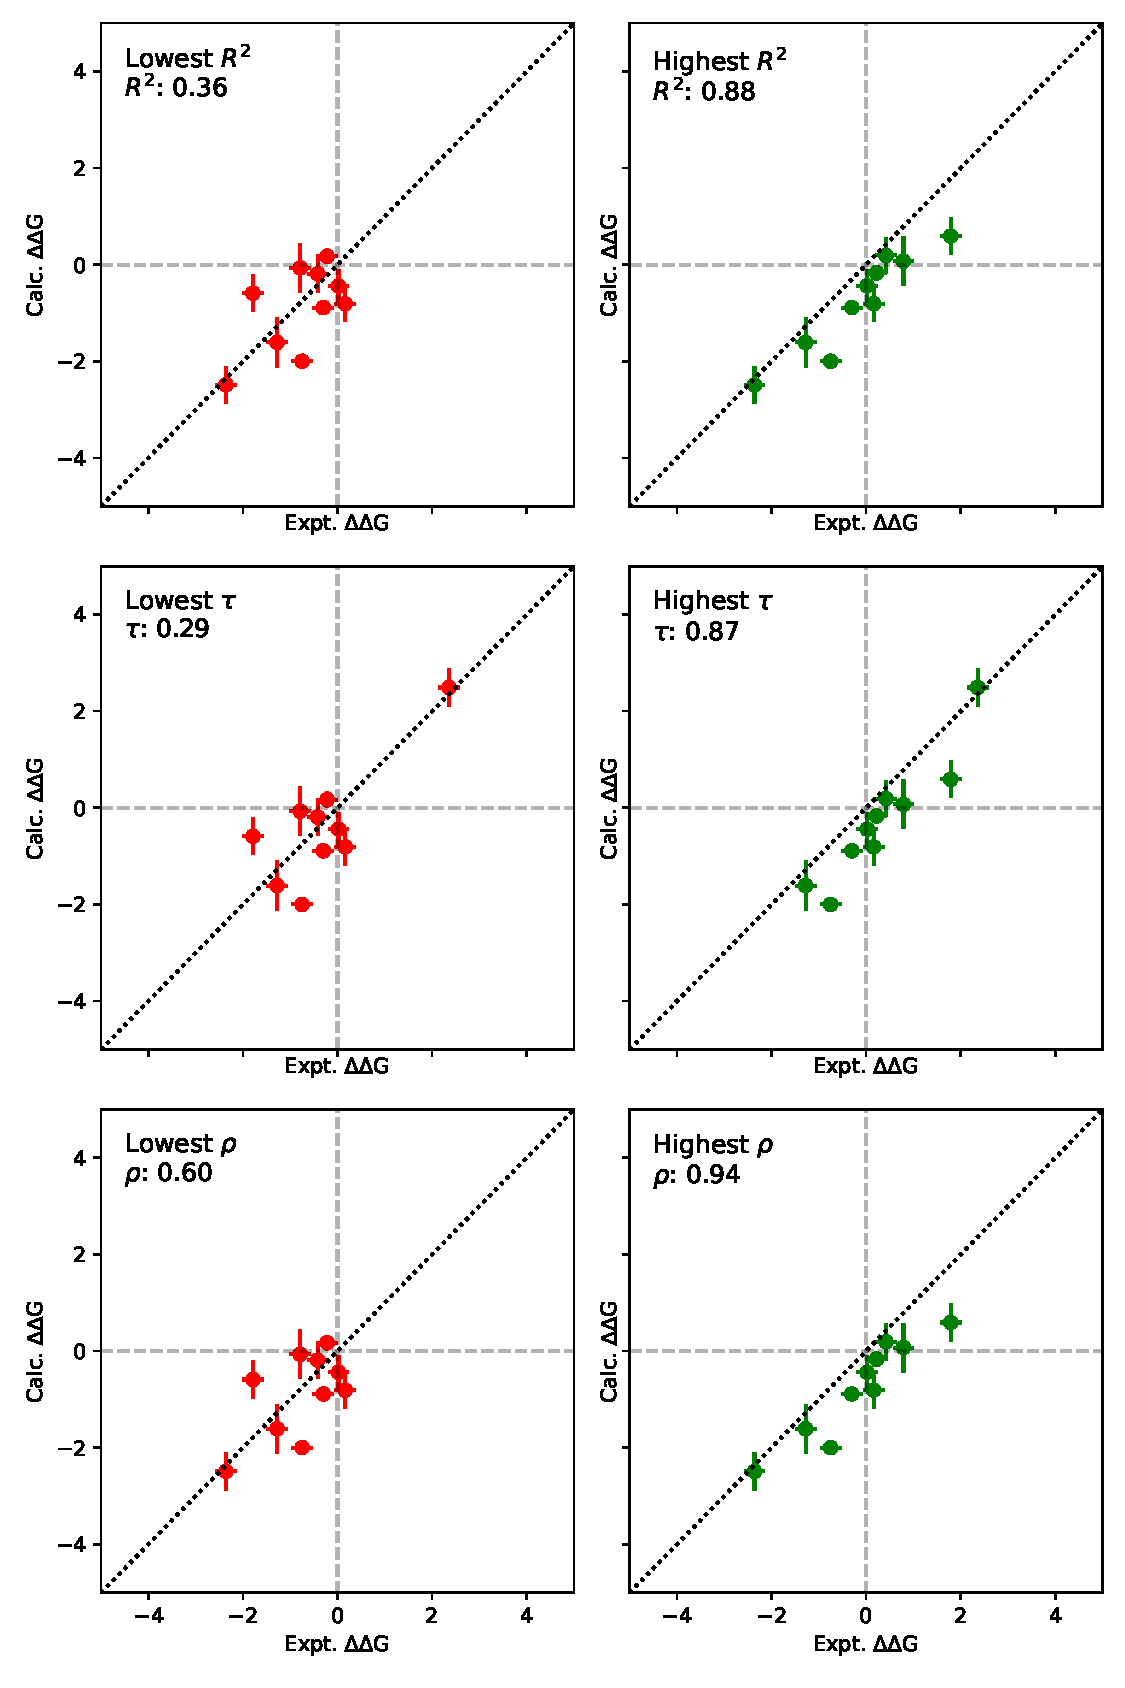
\includegraphics[width=0.95\linewidth]{figures/reporting/relativeissuesB.pdf}
    \caption{\textbf{Using correlation statistics with relative free energy results are unreliable.} For a set of $N$ datapoints, there are $\frac{2^N}{2}$ possible permutations in the sign for the datapoints, where the changes in sign results in a range of possible statistics from the same underlying data. For a set of 10 example relative free energies, the distribution of possible values ($\frac{2^{10}}{2} = 512$) for $R^2$, Kendall $\tau$ and $\rho$ are illustrated in the violin plot. The order of permutations that result in the highest (green) and lowest (red) correlation statistic are shown 
below, for $R^2$, Kendall $\tau$ and $\rho$, which illustrates how varied the correlation statistics for for the same relative free energy results can be achieved by simply using different definitions of relative 'directions' for various edges. For this reason, best practise is to avoid reporting correlation statistics for the reporting of relative free energy calculations, and using accuracy  statistics such as RMSE and MUE instead.}
    \label{fig:changing-corr}
\end{figure}

One mistake that is commonly made, is the use of correlation-type statistics for the benchmarking of relative free energy calculations. As relative calculations are pairwise comparisons between ligands, the direction, or sign of the calculation is arbitrary. If a ligand $A$ is 2 kcal mol$^{-1}$ higher affinity than ligand $B$, this could equally be plotted and reported as ligand $B$ being -2 kcal mol$^{-1}$ lower affinity than ligand $A$. The consequence of the possible inversion of data points can shift the correlation statistics, despite the underlying data being consistent. The same set of data points can give a range of statistical results depending on arbitrary sign-flips in the data set, where there are $\frac{2^N}{2}$ possible permutations for a set of $N$ relative free energies. While the size of this issue can be affected by the number, range and accuracy of the data points, this can still be problematic, as illustrated in Figure \ref{fig:changing-corr}. If a clear protocol is used, such as mapping all of the results to either be all positive or all negative, or plotting both $A \rightarrow B$ and $B \rightarrow A$ then the statistics quoted will be reproducible, however it is our recommendation to avoid correlation statistics for relative free energy results.

Additionally, correlation statistics, which are appropriate for reporting absolute free energy results, can be sensitive to the number of data points, and the range that they cover, as illustrated in Section \ref{sec:affinities}, Figure ~\ref{fig:N_CI}. This can be exacerbated by experimental uncertainties, which is covered in Section ~\ref{sec:affinities}. Some statistical measures are available that attempt to capture the inherent experimental range in the analysis, such as GRAM ~\cite{cui2019gram} and relative root-mean-squared error (RRMSE). As the number, dynamic range, and experimental uncertainty can all limit the maximum achievable correlation and confidence intervals, it is worth assessing these values \textit{a priori} when deciding if a particular protein-ligand dataset is appropriate for a benchmark (see Section \ref{sec:affinities}).


%-----------------------------------------------------------
\subsubsection{Bootstrapping is a reliable method for determining confidence intervals for statistics}
%-----------------------------------------------------------

While statistics are a useful measure of the performance of a method, it is also important to understand how accurate those measures are themselves. Is a MUE of 1.2 kcal mol$^{-1}$ much better than 1.3 kcal mol$^{-1}$? Would the performance be likely to change on the addition of new ligands in the series? Is the R$^2$ being heavily leveraged by a handful of outliers? Performing bootstrap analysis allows for confidence intervals to be placed on the statistics, and for these questions to be answered with some confidence. A MUE of 1.2 (0.6) kcal mol$^{-1}$ is not statistically different than a MUE of 1.3 (0.5) kcal mol$^{-1}$. Bootstrap analysis provides a measure of accuracy to the statistics through random sampling with replacement. Bootstrapping should be performed on the data used to compute the statistic reported --- for relative free energies this illustrate how sensitive the statistics are to the edges chosen, and for absolute free energies: the sensitivity to the ligands in the set. The statistical error for each data point should be incorporated in the bootstrap estimate, where bootstrapping is performed by taking a sample from each data point using its associated variance. It is best practise to report the bootstrapped statistical errors alongside data as 95\% confidence intervals to appropriately evaluate the performance of a particular method, and identify if improvements or changes to a model are statistically significant.

%\subsubsection{The maximum achievable computational accuracy is limited by the accuracy of the experimental data}\label{section:expt-accuracy}

%Quantifying the experimental uncertainty is necessary for understanding the upper-limit of feasible accuracy for a model~\cite{brown2009healthy}. Understanding this is both useful for fair comparison between methods, and for conveying the reliability of a model to medicinal chemists~\cite{griffen2020chemists}. Building predictive models becomes more difficult with (a) a small experimental dynamic range and (b) large experimental uncertainties. It is useful to understand the upper limit of success a computational method can have for a set of experimental results;

%\begin{equation}\label{eqn:r2max}
%    R^2_{\mathrm{max}} = 1 - (\frac{\sigma(\mathrm{measurement\,  error})}{\sigma(\mathrm{affinity})}) ^2,
%\end{equation}

%where $R^2_{\mathrm{max}}$ is the highest achievable $R^2$ for a dataset with a standard deviation of affinities ($\sigma(\mathrm{affinity})$) and an experimental uncertainty of  $\sigma(\mathrm{measurement \, error})$~\cite{sheridan2020experimental}.

%The primary publication of the experimental results is typically the best source of experimental uncertainty as cited affinities may occasionally be subject to rounding differences or unit errors~\cite{kramer2012experimental}. Errors quoted will likely to be an estimate of the repeatability of the assay, rather than true, independent reproducibility. Publications with essential experimental controls reported --- such as incubation time and concentration regime to demonstrate equilibrium --- can add confidence to the reported affinity, however these may be performed and not reported~\cite{jarmoskaite2020measure}. Meta-analyses of both repeatability~\cite{sheridan2020experimental} and reproducibility~\cite{kramer2012experimental} found errors of 0.3-0.4 log units (0.43-0.58 kcal mol$^{-1}$) and 0.44 (0.64 kcal mol$^{-1}$) log units respectively. These values provide a guideline for experimental error, if none is provided. It is not recommended to validate computational methods against experimental values obtained from a combination of sources if avoidable.\\

%If an experimental uncertainty of 0.64 kcal mol$^{-1}$ is assumed for a dataset with a standard deviation of affinity of 1.25 kcal mol$^{-1}$, using Equation \ref{eqn:r2max} an upper-limit R$^2_{\mathrm{max}}$ of 0.74 should be achievable.

%%%%%%%%%%%%%%%%%%%%%%%%%%%%%%%%%%%%%%%%%%%%%%%%%%%%%%%%%%%%
\section{Conclusions}
\label{sec:conclusion}
%%%%%%%%%%%%%%%%%%%%%%%%%%%%%%%%%%%%%%%%%%%%%%%%%%%%%%%%%%%%

Methods for binding free energy calculations have been continuously developed over the last decades and are increasingly used both in academic research as well as pharmaceutical industry applications in structure based drug discovery~\cite{sherborne_collaborating_2016, gapsysLargeScaleRelative2020,schindler_largescale_2020}, making their validation and benchmarking particularly crucial. 
%
A robust and transparent assessment is required to probe the various aspects of binding free energy calculations for prospective applications.  Potential aspects to be benchmarked comprise but are not limited to
(a) alternative inputs (e.g. different X-ray structures of the same target),
(b) alternative ways to prepare the input (e.g. different ligand alignment protocols),
(c) alternative model representations (e.g. different force field parameters),
(d) alternative calculation setups (e.g. perturbation map), and
(e) alternative calculation protocols (e.g. sampling methods).
%

In order to reliably benchmark methods, we provide best practices recommendations for setting up benchmark calculations.
This setup begins with the appropriate choice of experimental inputs and data, which includes 
the choice of target(s) and ligands (Section \ref{sec:dataset}). We require both
structural information (Section \ref{sec:struct_data}) and 
affinity data (Section \ref{sec:affinities}.
This input information needs to be adequately prepared to generate simulation inputs (Section \ref{sec:prep}) before the systems are simulated with a specific choice of 
software, 
calculation setup, and 
simulation protocol. Here, we made a variety of recommendations as to how to select and prepare systems for benchmarking.

Benchmarking also requires analysis and comparison with experiment, thus we also recommend standard reporting procedures (Section~\ref{sec:analysis}). These provide a mechanism to assess the accuracy of the calculations, present the results and compare to calculations done with other methods. These standard procedures will make it far easier to compare results across studies done by different researchers or using different tools.

Our recommendations are exemplified in publicly available tools for the analysis of calculations (github.com/openforcefield/arsenic)
and a living protein-ligand benchmark dataset (github.com/openforcefield/PLBenchmarks).
%

Here, we also provide a proposed living benchmark set. This set is living in the sense that we expect it to be subject to ongoing updates, curation, and improvement -- both by ourselves and by the community, and we welcome community input via the GitHub issue tracker at [where?]. Additionally, further curation is clearly necessary as our recommendations are in part not fulfilled in the initial version of this benchmark dataset. This is in part because we have begun from previously used benchmark sets and are beginning the curation process, but also because it is difficult to find large and accurate experimental data sets meeting all the desired characteristics. Thus, in our initial set, the relevant issues are annotated and we expect the benchmark set to evolve to better meet the recommendations given here.

We hope that our recommended best practices will be adopted and extended by the community, and we believe that these best practices will ultimately help advance the accuracy, applicability and availability of binding free energy calculations. 

%%%%%%%%%%%%%%%%%%%%%%%%%%%%%%%%%%%%%%%%%%%%%%%%%%%%%%%%%%%%
\section{Checklists}
\label{sec:checklists}
%%%%%%%%%%%%%%%%%%%%%%%%%%%%%%%%%%%%%%%%%%%%%%%%%%%%%%%%%%%%

\begin{Checklists*}

\begin{checklist}{Choose Suitable Protein Structures for Benchmarking}
\textbf{Find experimental structural data: Section~\ref{sec:struct_data}}

    \textbf{Global criteria}
    \begin{itemize}
        \item Select the best available structure (coordinate error < 0.7)
        \item Ensure experimental data is available, i.e. electron/neutron density or cyro EM map
        \item Ensure the reported $Rfree < 0.45$ when resolution $\le 3.5 \AA$
        \item Check that the reported difference between R and Rfree $\le 0.05$
        \end{itemize}
    \textbf{Local criteria}
    \begin{itemize}
        \item Identify ligand atoms where there are crystal packing atoms within 6 $\AA$
        \item Confirm that the ligand has at least partial density (check visually or RSCC > 0.90) and the density is adequate to confirm ligand presence and binding mode
        \item All ligand and active site atoms with occupancy <1.0 are identified
        \item Identify active site atoms with partial density and ensure these are acceptable and not key contacts
        \item Confirm whether crystallographic waters are resolved
        \item Identify any alternate conformations for ligand and active site atoms 
        \item Confirm that this is not a covalent ligand as deposited, and is also not likely to have reacted to become one
        \item Are there crystal contacts? 
        \item Check for any missing loops or residues and side chain atoms in the structure and confirm these are not near the binding site/not key for the study
    \end{itemize}
% \item aspects to be considered beyond the quality of the structure (see also structure preparation, Sect. \ref{sec:prep}
%     \begin{itemize}
%     \item Structure (also the binding mode!) could be deformed due to crystal contacts, additives, experimental temperature,... Can you assume the structure in the crystalline form is representative of the biologically active conformation? 
%     \item Content of the structure: is the small molecule (or a closely related one) bound? 
%     \item Are there cofactors or cobinders which should be included to model the natural environment of the protein?
%     \item Can we model the measurement conditions, temperature, ion concentration, other additives?
%     \item Can we model the natural environment (ion concentration, cofactors, membranes, ...)?
%     \end{itemize}
% \item If these requirements are not met, it does not necessarily mean that the data is not usable and  the results will be bad. A structure not meeting the requirements just needs more manual work by --- ideally an experienced --- user. Unresolved areas can be modelled with nowadays tools and knowledge about atom interactions.
% \item Collective intelligence could be a way to mitigate the influence of individuals to the prepared input structures of a benchmark set. On a platform, other scientists could suggest changes to structures and updated versions could be deposited, increasing the quality of the benchmark set. Endorsement and rating of deposited structures could increase the trust into specific structures and the database in general. 
\end{checklist}

\begin{checklist}{Ensure Affinity Data is Adequate for Benchmarking}
\textbf{Find experimental affinity data: Section~\ref{sec:affinities}}
    \begin{itemize}
    \item Single source data.
    \item Extract binding data from original source and convert carefully.
    \item Remove data points outside detection limits.
    \item Ideally data should be from biophysical assays. With functional assays, more care must be taken.
    \item Assess dataset quality in terms of number of datapoints, experimental affinity range and experimental error to know the maximally achievable precision.
    \end{itemize}
\end{checklist}

\end{Checklists*}


\begin{Checklists*}
\begin{checklist}{Prepare the System with Care Because Failures Here are Crucial}
\textbf{Prepare structural data for simulation: Section~\ref{sec:prep}}
    \begin{itemize}
        \item Assess which domains of the X-ray structure are needed and retain domains present in the experimental study, unless it is known that further simplifications can be made without affecting accuracy
        \item Check other components of the structure and remove if they do not affect your simulation or system, such as: cofactors, structural waters, other ligands, PTMs.
        \item Split the protein and ligand structures to prepare separately.\\
        \textbf{Protein preparation}
    \begin{itemize}
                \item Add caps if needed.
                \item If possible, model missing loops, if loops are too long (> 15 to 20 residues) or too mobile, consider capping the ends and adding restraints, or modeling a short GLY loop that links both ends. These must not be in the binding site.
                \item Inspect for  side chain flips of side chains which can fit density similarly when reoriented (HIS, ASN, GLN); confirm that the orientations chosen lead to preferred interactions with the ligand. Evaluate alternate placements if necessary.
                \item Check the protonation states of the ligand and receptor, again checking in the context of the interactions that would be formed with the ligand.
    \end{itemize}
        \textbf{Ligand preparation}
    \begin{itemize}
            \item Check the chemical structure is correct (bond orders, stereochemistry).
            \item Align the ligand series based on conformations of (X-ray) reference compound(s).
            \item Check tautomer and ionization states. Determine whether multiple possibilities need to be considered
            \item Check whether alternate rotamers may need to be considered after alignment to reference compound(s)
    \end{itemize}
    \end{itemize}
        \textbf{System preparation}
    \begin{itemize}
        \item Assemble the protein and ligand, solvate or embed in a membrane. 
        \item Add ions; use an appropriate salt concentration to model the assay
        \item Equilibrate the system.
    \end{itemize}
\end{checklist}

\begin{checklist}{Carefully Select Appropriate Simulation Details}
\textbf{Choose simulation setup: Section~\ref{sec:alchemical_prep}}
    \begin{itemize}
        \item Choose absolute vs. relative calculations.
        \item Choose topology approach and alchemical pathway.
        \item Choose sampling protocol.
        \item Plan a perturbation map if calculations are relative
    \end{itemize}
\end{checklist}
\end{Checklists*}


\begin{Checklists*}
\begin{checklist}{Present Graphs of Results in a Consistent Manner}
\textbf{Presenting results in an appropriate format: Section~\ref{sec:plotting_results}}
\begin{itemize}
\item Clearly label the data with titles, legends, and captions.
\item Plot results with the dependent variable (calculated) on y-axis, and the independent variable (experimental) on the x-axis. 
\item Ensure that the data are reported in the same units on both axes, and labelled. The scale of the axis in real space should be consistent, such that a 1 cm change on the x-axis corresponds to the same change in affinity to 1 cm on the y-axis.
\item Plot only one target per plot, unless specifically looking at selectivity.
\end{itemize}
\end{checklist}

\begin{checklist}{Use Careful Statistical Analysis to Quantify Performance}
\textbf{Quantifying the success of a method: Section~\ref{sec:statistical_analysis}}
\begin{itemize}
\item Identify which metrics are appropriate for your method. Statistics that measure accuracy, such as RMSE and MUE, are commonplace; correlation statistics are appropriate for absolute free energies, but not relative free energies.
\item Bootstrap statistics to provide confidence intervals. 
\item Provide confidence intervals for all reported values and avoid overinterpreting results given these intervals
\end{itemize}
\end{checklist}


\end{Checklists*}




%%%%%%%%%%%%%%%%%%%%%%%%%%%%%%%%%%%%%%%%%%%%%%%%%%%%%%%%%%%%
\section{Author Contributions}
%%%%%%%%%%%%%%%%%%%%%%%%%%%%%%%%%%%%%%%%%%%%%%%%%%%%%%%%%%%%
% This section must describe the actual contributions of
% author. Since this is an electronic-only journal, there is
% no length limit when you describe the authors' contributions,
% so we recommend describing what they actually did rather than
% simply categorizing them in a small number of
% predefined roles as might be done in other journals.
%
% See the policies ``Policies on Authorship'' section of https://livecoms.github.io
% for more information on deciding on authorship and author order.
%%%%%%%%%%%%%%%%%%%%%%%%%%%%%%%%%%%%%%%%%%%%%%%%%%%%%%%%%%%%

(Explain the contributions of the different authors here)
ASJSM: Wrote Sec.~\ref{sec:alchemical_prep} and created Fig.~\ref{fig:map} and Fig.~\ref{fig:protocols}. 
GT: Wrote introduction and dataset selection section, edited the final manuscript.
DFH: Coordinated the writing, wrote the structural data section and conclusions, contributed to most sections.
GLW: Generated the data for Table 1 and contributed to the text in the structural data section.


% We suggest you preserve this comment:
For a more detailed description of author contributions,
see the GitHub issue tracking and changelog at \githubrepository.


%%%%%%%%%%%%%%%%%%%%%%%%%%%%%%%%%%%%%%%%%%%%%%%%%%%%%%%%%%%%
\section{Other Contributions}
%%%%%%%%%%%%%%%%%%%%%%%%%%%%%%%%%%%%%%%%%%%%%%%%%%%%%%%%%%%%
% You should include all people who have filed issues that were
% accepted into the paper, or that upon discussion altered what was in the paper.
% Multiple significant contributions might mean that the contributor
% should be moved to authorship at the discretion of the a
%
% See the policies ``Policies on Authorship'' section of https://livecoms.github.io for
% more information on deciding on authorship and author order.
%%%%%%%%%%%%%%%%%%%%%%%%%%%%%%%%%%%%%%%%%%%%%%%%%%%%%%%%%%%%

(Explain the contributions of any non-author contributors here)
% We suggest you preserve this comment:
For a more detailed description of contributions from the community and others, see the GitHub issue tracking and changelog at \githubrepository.

\section{Potentially Conflicting Interests}
%%%%%%%
%Declare any potentially competing interests, financial or otherwise
%%%%%%%

%Declare any potentially conflicting interests here, whether or not they pose an actual conflict in your view.
DLM serves on the scientific advisory board for OpenEye Scientific Software and is an Open Science Fellow with Silicon Therapeutics.

\section{Funding Information}
%%%%%%%
% Authors should acknowledge funding sources here. Reference specific grants.
%%%%%%%
JDC acknowledges support from NIH grant P30 CA008748.
We appreciate the financial support of the Open Force Field Consortium (\url{https://openforcefield.org}), and the National Institutes of Health (NIGMS R01GM132386 and R01GM108889).
HEBM acknowledges support from a Molecular Sciences Software Institute Investment Fellowship and Relay Therapeutics. 


\section*{Author Information}
\makeorcid

\bibliography{livecoms-sample}

%%%%%%%%%%%%%%%%%%%%%%%%%%%%%%%%%%%%%%%%%%%%%%%%%%%%%%%%%%%%
%%% APPENDICES
%%%%%%%%%%%%%%%%%%%%%%%%%%%%%%%%%%%%%%%%%%%%%%%%%%%%%%%%%%%%

%\appendix


\end{document}
